%%%%%%%%%%%%%%%%%%%%%%%%%%%%%%%%%%%%%%%%%
% Short Sectioned Assignment LaTeX Template Version 1.0 (5/5/12)
% This template has been downloaded from: http://www.LaTeXTemplates.com
% Original author:  Frits Wenneker (http://www.howtotex.com)
% License: CC BY-NC-SA 3.0 (http://creativecommons.org/licenses/by-nc-sa/3.0/)
%%%%%%%%%%%%%%%%%%%%%%%%%%%%%%%%%%%%%%%%%

% \documentclass[paper=a4, fontsize=11pt]{scrartcl} % A4 paper and 11pt font size
\documentclass[12pt, a4paper, openany]{book}
\usepackage[T1]{fontenc} % Use 8-bit encoding that has 256 glyphs
\usepackage{fourier} % Use the Adobe Utopia font for the document - comment this line to return to the LaTeX default
\usepackage[utf8]{inputenc}
\usepackage{listings} % para insertar código con formato similar al editor
\usepackage[spanish, es-tabla]{babel} % Selecciona el español para palabras introducidas automáticamente, p.ej. "septiembre" en la fecha y especifica que se use la palabra Tabla en vez de Cuadro
\usepackage{url} % ,href} %para incluir URLs e hipervínculos dentro del texto (aunque hay que instalar href)
\usepackage{graphics,graphicx, float} %para incluir imágenes y colocarlas
\usepackage[gen]{eurosym} %para incluir el símbolo del euro
\usepackage{cite} %para incluir citas del archivo <nombre>.bib
\usepackage{enumerate}
\usepackage{hyperref}
\usepackage{graphicx}
\usepackage{tabularx}
\usepackage{booktabs}
\usepackage{float}
\usepackage{amsmath}
\usepackage{fontawesome}
\usepackage[table,xcdraw]{xcolor}

\hypersetup{
	colorlinks=true,	% false: boxed links; true: colored links
	linkcolor=black,	% color of internal links
	urlcolor=cyan		% color of external links
}
\usepackage{fancyhdr} % Custom headers and footers
\pagestyle{fancyplain} % Makes all pages in the document conform to the custom headers and footers
\fancyhead[L]{} % Empty left header
\fancyhead[C]{} % Empty center header
\fancyhead[R]{} % My name
\fancyfoot[L]{} % Empty left footer
\fancyfoot[C]{} % Empty center footer
\fancyfoot[R]{\thepage} % Page numbering for right footer
%\renewcommand{\headrulewidth}{0pt} % Remove header underlines
\renewcommand{\footrulewidth}{0pt} % Remove footer underlines
\setlength{\headheight}{15.0pt} % Customize the height of the header
%\renewcommand{\familydefault}{\sfdefault}
\usepackage{titlesec, blindtext, color}


\definecolor{gray75}{gray}{0.75}
\definecolor{lightpurple}{HTML}{eeddff}
\definecolor{deeppurple}{HTML}{c58cff}

\newcommand{\hsp}{\hspace{20pt}}
\titleformat{\chapter}[hang]{\Huge\bfseries}{\thechapter\hsp\textcolor{gray75}{|}\hsp}{0pt}{\Huge\bfseries}
\setcounter{secnumdepth}{4}
\usepackage[Bjornstrup]{fncychap}

\renewcommand\DOCH{%
  \settowidth{\py}{\CNoV\thechapter}
  \addtolength{\py}{-10pt}
  \fboxsep=0pt%
  \colorbox{lightpurple}{\rule{0pt}{40pt}\parbox[b]{\textwidth}{\hfill}}%
  \kern-\py\raise20pt%
  \hbox{\color{deeppurple}\CNoV\thechapter}\\%
}

\renewcommand\DOTI[1]{%
  \nointerlineskip\raggedright%
  \fboxsep=\myhi%
  \vskip-1ex%
  \colorbox{lightpurple}{\parbox[t]{\mylen}{\CTV\FmTi{#1}}}\par\nobreak%
  \vskip 40pt%
}

\renewcommand\DOTIS[1]{%
  \fboxsep=0pt
  \colorbox{lightpurple}{\rule{0pt}{40pt}\parbox[b]{\textwidth}{\hfill}}\\%
  \nointerlineskip\raggedright%
  \fboxsep=\myhi%
  \colorbox{lightpurple}{\parbox[t]{\mylen}{\CTV\FmTi{#1}}}\par\nobreak%
  \vskip 40pt%
 }


\begin{document}

	% Plantilla portada UGR
	\begin{titlepage}
\newlength{\centeroffset}
\setlength{\centeroffset}{-0.5\oddsidemargin}
\addtolength{\centeroffset}{0.5\evensidemargin}
\thispagestyle{empty}

\noindent\hspace*{\centeroffset}\begin{minipage}{\textwidth}

\centering

\includegraphics[width=0.9\textwidth]{logos/logo_ugr.jpg}\\[1.4cm]

\textsc{ \Large TRABAJO FIN DE GRADO\\[0.2cm]}
\textsc{ GRADO EN INGENIERIA INFORMATICA}\\[1cm]

\center{\Huge\bfseries Control de elementos  }
\center{\Huge\bfseries de un automóvil mediante}
\center{\Huge\bfseries  un sistema empotrado} 
\noindent\rule[-1ex]{\textwidth}{1pt}\\[3.5ex]

\end{minipage}

\vspace{2.5cm}
\noindent\hspace*{\centeroffset}
\begin{minipage}{\textwidth}
\centering

\textbf{Autor}\\ {Sheila Martínez Gómez}\\[2.5ex]
\textbf{Director}\\ {Jesús González Peñalver}\\[2cm]

\includegraphics[width=0.3\textwidth]{logos/etsiit_logo.png}\\[0.1cm]
\textsc{Escuela Técnica Superior de Ingenierías Informática y de Telecomunicación}\\

\end{minipage}
\end{titlepage}


	% Plantilla prefacio UGR
	\thispagestyle{empty}

\begin{center}
{\large\bfseries Control de elementos de un automóvil \\ mediante un Sistema Empotrado }\\
\end{center}
\begin{center}
Sheila Martínez Gómez\\
\end{center}

%\vspace{0.7cm}

\vspace{0.5cm}
\noindent\textbf{Palabras clave}: \textit{software libre, sistema empotrado, ECU, microcontrolador, centralita, RTOS, automoción}
\vspace{0.7cm}

\noindent\textbf{Resumen}\\
	

\cleardoublepage

\begin{center}
	{\large\bfseries Same, but in English}\\
\end{center}
\begin{center}
	Student's name\\
\end{center}
\vspace{0.5cm}
\noindent\textbf{Keywords}: \textit{open source, embedded system, ECU, microcontroller,RTOS, automotive}, \textit{floss}
\vspace{0.7cm}

\noindent\textbf{Abstract}\\


\cleardoublepage

\thispagestyle{empty}

\noindent\rule[-1ex]{\textwidth}{2pt}\\[4.5ex]

D. \textbf{Tutora/e(s)}, Profesor(a) del ...

\vspace{0.5cm}

\textbf{Informo:}

\vspace{0.5cm}

Que el presente trabajo, titulado \textit{\textbf{Chief}},
ha sido realizado bajo mi supervisión por \textbf{Estudiante}, y autorizo la defensa de dicho trabajo ante el tribunal
que corresponda.

\vspace{0.5cm}

Y para que conste, expiden y firman el presente informe en Granada a Junio de 2018.

\vspace{1cm}

\textbf{El/la director(a)/es: }

\vspace{5cm}

\noindent \textbf{(nombre completo tutor/a/es)}

\chapter*{Agradecimientos}






	% Índice de contenidos
	\newpage
	\tableofcontents

	% Índice de imágenes y tablas
	\newpage
	\listoffigures

	% Si hay suficientes se incluirá dicho índice
	\listoftables 
	\newpage

	% Introducción 
	\chapter{Introducción}

Este proyecto es software libre, y está liberado con la licencia \cite{gplv3}.

\section{Motivación}

\subsection{La complejidad de los automóviles actuales}

Debido a la evolución tan rápida de los sistemas de los vehículos en las últimas décadas, nos encontramos con multitud de problemas que antes no habríamos tenido que experimentar, pero también nos otorgan una gran cantidad de información acerca de los diversos módulos del vehículo. 
Esto nos dota de una mayor seguridad a la hora de poder comprobar, de un simple vistazo, si nuestro automóvil está en buen estado, pero... ¿Cómo manejar todos esos sistemas de manera simultánea y mostrárselo al conductor? 



\subsection{Los sistemas empotrados en la sociedad actual}

Los sistemas empotrados forman parte de nuestra vida diaria, aunque en la mayoría de los casos nunca llegamos a verlos en sí mismos, sino ocultos en objetos cotidianos como los microondas, las vitrocerámicas, etcétera. Basan su funcionamiento en obtención de señales mediante sensores que dan información sobre el entorno y, tras procesar esos datos en un lapso de tiempo normalmente determinado, responden mediante un actuador dándonos la funcionalidad que buscamos. 


\newpage
\section{Estructura del trabajo}

El trabajo está compuesto de los siguientes capítulos: 

\begin{itemize}
    \item \textbf{Capítulo 1} - Introducción: Capítulo actual, en el que se habla de las bases del trabajo que se va a realizar.
    \item \textbf{Capítulo 2} - Descripción del problema: En este capítulo se hablará del objetivo del trabajo, de las restricciones que se van a encontrar y de los requisitos para llevarlo a cabo.
    \item \textbf{Capítulo 3} - Antecedentes: En este apartado se hablará de la tecnología de las ECU, y de toda la información necesaria para tener una visión completa del conjunto, todo esto para poder realizar el trabajo práctico con suficientes conocimientos.
    \item \textbf{Capítulo 4} - ... [pend]
    \item \textbf{Capítulo 5} - ... [pend]
    \item \textbf{Capítulo 6} - ... [pend]
    \item \textbf{Capítulo 7} - ... [pend]
\end{itemize}


	% Descripción del problema y hasta donde se llega
	\chapter{Descripción del problema}
\section{El problema}

Debido a los avances nombrados en la introducción, la complejidad que supone entender cómo pueden funcionar todos los módulos que componen los vehículos actuales, puesto que son sistemas demasiado intrincados para que alguien que no pertenezca al campo de estudio/trabajo de estos puedan tener más que una imagen general del conjunto. \\

Podemos resumir las cuestiones que conforman el problema en los siguientes puntos:

\begin{itemize}
    \item A medida que avanza la tecnología, los vehículos se apoyan en más sistemas informáticos y ayudas electrónicas, alejándose de la simpleza de los automóviles antiguos en estos campos.

    \item Las empresas mantienen estos sistemas con un diseño propietario, oculto al público general, por lo que no podemos siquiera observar sus métodos.

    \item A pesar de estas desventajas, los vehículos se están actualizando a pasos agigantados cada año, y comprender las partes más importantes del conjunto podría ser muy útil para el usuario medio de estos en su día a día.

    \item Este proyecto puede aportar un enfoque dinámico para un primer acercamiento de la juventud al automovilismo actual.
\end{itemize}


\section{Solucion propuesta}

La solución que se propone es la creación de un sistema que emule la ECU de un vehículo, pero de manera simplificada, mediante un sistema empotrado que soporte un sistema operativo de tiempo real para poder atender a todas las peticiones en un tiempo de respuesta acotado. 

Para mantener esta Unidad de Control Electrónico (ó \textit(ECU)) accesible y poder desarrollar el proyecto sin tener que hacer una gran inversión económica, utilizaremos software de código abierto así como componentes de bajo coste para la construcción.

Si la temporización nos lo permite, también se podrán implementar estos sistemas en una maqueta de un vehículo, además de visualizar los valores de los módulos en un programa en un computador remoto.  


\section{Restricciones}
Pasta
NO podemos abarcar todo en una maqueta etc.
\section{Objetivos}



\begin{itemize}
    \item ¿Qué sistemas se podrían \"emular\" respecto a los vehículos reales, y con qué \textit{hardware}?
    \item ¿Con qué \textit{hardware} podemos afrontar la gestión, recepción y procesamiento de información de los diversos sistemas?
    \item ¿Cómo gestionar el \textit{firmware} y el \textit{software} para que realicen las tareas necesarias?
    \item Tras obtener los datos de estos sistemas, ¿Cómo filtrar la información para mostrarla en una interfaz, y de qué tipo?
\end{itemize}

\subsection{Objetivos de Investigación y Aprendizaje}
\subsection{Objetivos de Diseño y Desarrollo}



	\chapter{Antecedentes}


\section{¿Qué es una ECU?}


Una ECU \textit{Electronic Control Unit} es un sistema empotrado, que consta de un microcontrolador especializado en la automoción. [1] (embitel.com) Permite, junto con el software y los protocolos de comunicación, y el conjunto de sensores y actuadores, controlar los sistemas eléctricos y subsistemas en un vehículo para su correcto funcionamiento. 
Esencialmente se encarga de recibir la información que le aportan los sensores acerca del entorno, procesar esa información para completar diversas tareas y, en muchos casos, enviar las directrices que se requieren a los actuadores de los componentes.\newline


\begin{figure}[h]
    \centering
    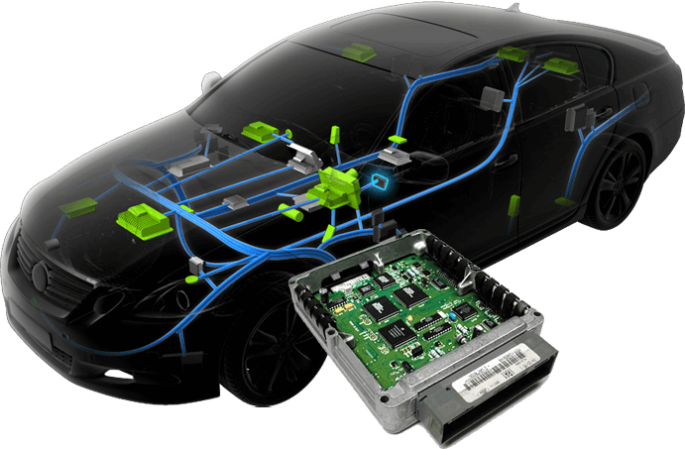
\includegraphics[width=0.5\textwidth]{imagenes/ECU_autotechdrive.png}
    \caption{Imagen de una ECU y su impacto en un vehículo. Extraído de: []}
\end{figure}


\subsection{Evolución e historia de la gestión de datos los vehículos}

Las siglas ECU no siempre han tenido el mismo significado. Inicialmente, cuando se comenzaron a utilizar (en torno a los años setenta), era para hablar de la unidad de control del motor \textit{\textbf{Engine Control Unit}}. Podemos desgajar los grandes cambios en lo siguiente[4]:

\begin{itemize}

    \item \textbf{Años 70} - Inicialmente eran dispositivos extremadamente simples, que solamente controlaban un par de solenoides en el \textbf{carburador}, el encargado de preparar la mezcla de aire y combustible en motores de gasolina, de manera que el vehículo pudiera obtener la máxima potencia de salida de la manera más eficiente.

    \begin{figure}[h]
        \centering
        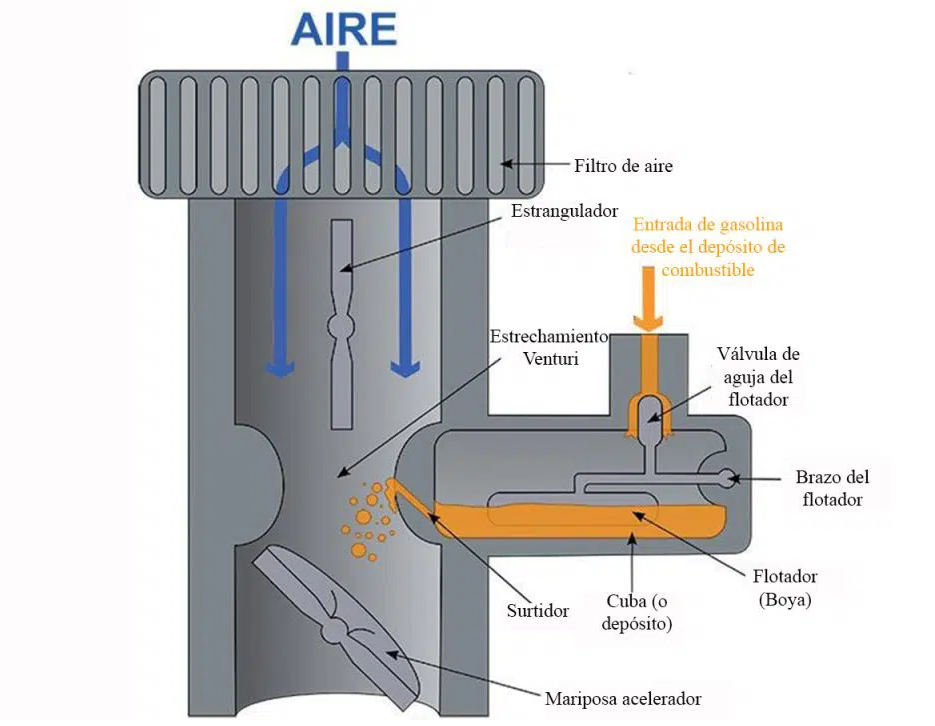
\includegraphics[width=0.5\textwidth]{imagenes/esquema_carburador.png}
        \caption{Imagen simplificada de un carburador sus partes. Extraído de: [5]}
    \end{figure}
 
    \item \textbf{Años 80} - En esta época se comenzaron a utilizar los \textbf{reguladores de presión de combustible}, un componente que busca controlar y mantener constante la presión del combustible. Permitió a los fabricantes de vehículos tener mayor control a la hora de no dañar otros componentes, tales como inyectores o los conductos del sistema en general [5]. En este punto, la unidad de control del motor ya era la principal responsable de los sistemas de combustión. También comenzaron a utilizar el \textbf{Control de Lambda} para modificar parámetros de la misma, y alcanzar una mayor eficiencia.

    \begin{figure}[h]
        \centering
        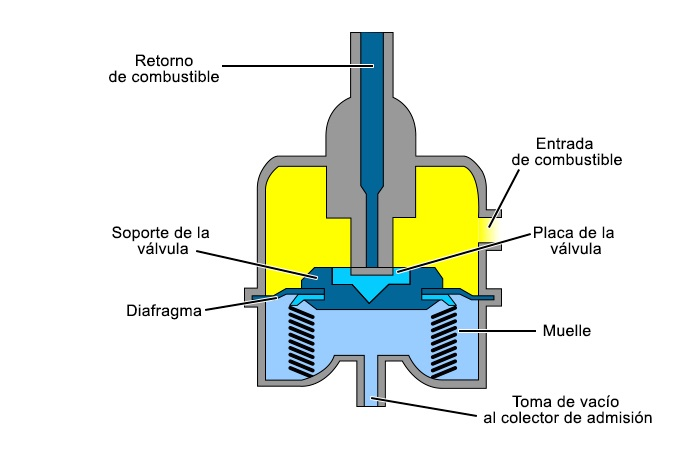
\includegraphics[width=0.6\textwidth]{imagenes/esquema_rpc.png}
        \caption{Imagen simplificada de un regulador de combustible y sus partes. Extraído de: [7]}
    \end{figure}


    \item \textbf{Años 90} - Las ECUs añadieron un conjunto de medidas para mejorar la seguridad en el vehículo, siendo el \textbf{ABS ó Antiblockiersystem} la más relevante. Esta tecnología, aún en uso en los vehículos actuales, se encarga de variar la fuerza de frenado al detectar mediante sensores de revoluciones en las ruedas, evitando así que estas se bloqueen y perdamos el control del vehículo. El uso de las ECUs se extiende hacia los motores diésel, teniendo un papel esencial en el desarrollo de los vehículos turbodiésel.

    \begin{figure}[h]
        \centering
        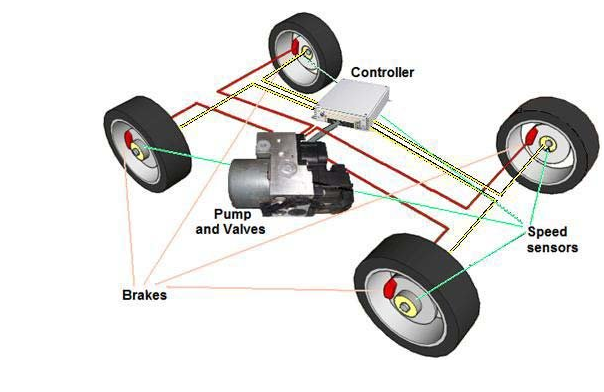
\includegraphics[width=0.5\textwidth]{imagenes/esquema_abs.png}
        \caption{Imagen simplificada del ABS y sus partes. Extraído de: [8]}
    \end{figure}
    
 
    \item \textbf{Años 2000} - Las unidades de control comienzan a incluir la tecnología \textit{\textbf{drive-by-wire}}, un formalismo para definir la sustitución de controles mecánicos tradicionales por sistemas electrónicos [9], así como también se añade control del turbo y sistemas para minimizar emisiones y cumplir con los protocolos pertinentes.
       

    \begin{figure}[h]
        \centering
        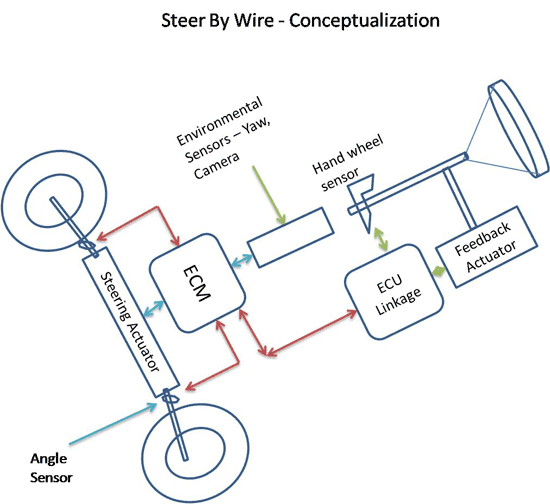
\includegraphics[width=0.5\textwidth]{imagenes/esquema_dbw.png}
        \caption{Conceptualización del sistema \textit{drive-by-wire}. Extraído de: [10]}
    \end{figure}
          

    \item \textbf{Años 2010-Actualidad} - La centralita del motor controla todo el sistema de mezcla del combustible, emisiones, refrigeración y sistemas de aceleración del vehículo. Dejan de ser dispositivos simples, ahora tienen cientos de entradas, decenas de sensores, y forman parte de un conjunto de ECUs (ya utilizando la acepción actual del término: \textit{Electronic Control Unit}), cada una focalizada en un conjunto de tareas, yendo desde el propio control del motor, hasta los sistemas de infoentretenimiento del vehículo. 
       

    \begin{figure}[h]
        \centering
        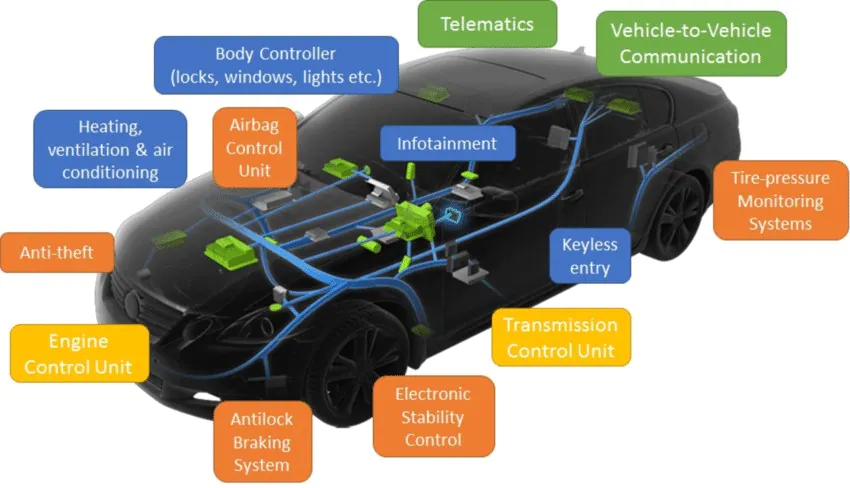
\includegraphics[width=0.5\textwidth]{imagenes/ECU_autotechdrive_completa.png}
        \caption{Representación de las distintas ECUs que controlan un vehículo. Extraído de: [11]}
    \end{figure}
\end{itemize}

\newpage
       
\begin{figure}[h]
    \centering
    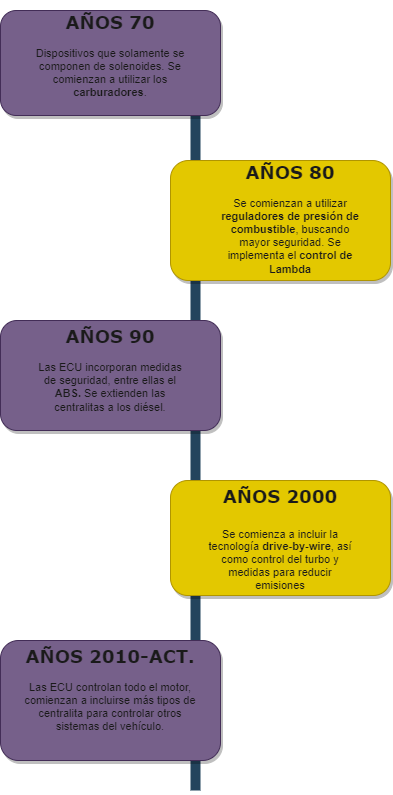
\includegraphics[width=0.54\textwidth]{imagenes/timeline_ECU.png}
    \caption{Linea temporal de las ECUs. Elaboración propia}
\end{figure}


\newpage


\subsection{Tipos de ECUs}
Como se ha visto en el anterior apartado, el significado de las siglas ECU ha variado con el tiempo, refiriéndose ahora a cada uno de los sistemas que controlan diversas partes del vehículo. A grandes rasgos, podemos hablar de los siguientes tipos[12]
\begin{itemize}
    \item \textbf{BCM - \textit{Body Control Module}}: Esta unidad controla tareas de índole variada, desde las luces, hasta el mecanismo de las ventanas, los retrovisores (si son motorizados), limpiaparabrisas, etc.
    \item \textbf{CCM - \textit{Climate Control Module}}: Este módulo se encarga de gestionar toda la climatización, temperatura, potencia de la bomba del aire acondicionado y calefacción.
    \item \textbf{ECM - \textit{Engine Control Module}}: Conocido antiguamente como ECU. Se encarga de gestionar todas las tareas del motor, ya mencionadas en el apartado anterior.
    \item \textbf{EBCM - \textit{Electronic Brake Control Module}}: Si el vehículo tiene un freno electrónico, este módulo es el encargado de su correcto funcionamiento.
    \item \textbf{ICM - \textit{Infotainment Control Module}}: Esta ECU controla todo lo relacionado con el infoentretenimiento, mayormente centrado en la tableta integrada del vehículo.
    \item \textbf{PSM - \textit{Power Steering Module}}: Este módulo gestiona las tareas que requiere la dirección para funcionar. Tiene una gran importancia, debido al uso de la dirección asistida en los vehículos actuales.
    \item \textbf{PCM - \textit{Powertrain Control Module}}: Esta ECU se encarga de la interconexión e interacción de los componentes que forman el \textbf{tren motriz}, el sistema que permite que la energía generada se transforme en movimiento sobre el terreno. Gestiona lo relacionado con el motor, la transmisión, los ejes, los diferenciales y la dirección del vehículo. 
    \item \textbf{SCM - \textit{Suspension Control Module}}: El objetivo de este módulo es controlar los sistemas de suspensión del vehículo.
    \item \textbf{TCM - \textit{Transmission Control Module}}: Este módulo controla todo lo relacionado con la transmisión, las marchas, el cambio y la entrega de potencia en las ruedas.
\end{itemize}
\newpage
\section{Diseño hardware de las centralitas}

Para tener un funcionamiento acorde a su importancia, las ECUs están constituidas por varios componentes, que serán los que se estudiarán en este apartado.

\begin{figure}[h]
    \centering
    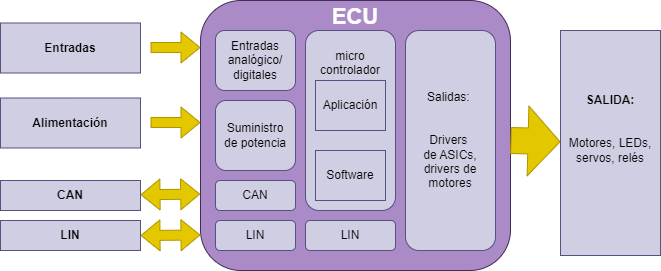
\includegraphics[width=0.70\textwidth]{imagenes/ECU_hardware.png}
    \caption{Componentes hardware de una ECU. Elaboración propia}
\end{figure}

\subsection{Procesador central}
El microcontrolador es la piedra angular de una centralita. Su tarea varía según el tipo de ECU que lo contenga, pero generalmente consiste en realizar todo el procesamiento de datos, así como hacer uso de las lineas de comunicación para recibir y enviar información a los subsistemas requeridos. \newline
Estos microcontroladores pueden interaccionar entre sí, aun perteneciendo a diferentes centralitas, por medio de \textbf{multiplexación}, así como también de los buses o protocolos de comunicación. Esta relación permite a un sistema valerse de otros para realizar una tarea, véase el siguiente ejemplo: 

\begin{enumerate}
    \item El usuario nota que hace demasiado calor en el vehículo, por lo que decide cambiar la temperatura en la tableta central del vehículo.
    \item Este sistema, controlado por el \textbf{ICM} (\textit{Infotainment Control Module}), recibe la entrada del usuario y envía una señal a la ECU que se encarga de la climatización (\textbf{CCM}).
    \item El módulo de climatización recibe la entrada y envía una señal a sus actuadores para encender el aire acondicionado.
\end{enumerate}


Respecto a la arquitectura del microcontrolador, existen diversas opciones, todas (o casi todas) ellas oscilando entre los 8 bits y los 32 bits, siendo estos últimos los más extendidos con el \textbf{Infineon Tri-core Microcontroller[19]}. Este micro se encarga de gestionar todas las tareas de emisiones y sistemas de combustión. 

La elección entre un chip u otro también se hace en base a las necesidades del sistema, puesto que algunos, como el tren de potencia y el control del vehículo requieren de un menor tiempo de respuesta y un mayor rendimiento, mientras que el infoentretenimiento no tiene tanta restricción al ser un \textbf{sistema de tiempo real blando} (incumplir el límite acotado del tiempo de respuesta no ocasiona daños personales o materiales)

\subsection{Memoria}

En una ECU, normalmente existen tres tipos de memoria, \textbf{ROM}, \textbf{RAM} y \textbf{PROM/EEPROM}. Cada una tiene un objetivo específico y unas restricciones asociadas:

\begin{itemize}
    \item \textbf{Memoria no volátil}: La ECU almacena en este tipo de memoria información que no se debe borrar una vez se apague el vehículo, como los datos del sistema y los del usuario (configuraciones, perfiles de conducción, etcétera.).
    \begin{itemize}
        \item \textbf{ROM}: Almacena información de programación que solo puede leer la ECU. Es de solo lectura, y su existencia es de vital importancia para el funcionamiento del vehículo.
        \item \textbf{PROM/EEPROM}: Este tipo de memoria está hecha por el fabricante, con el objetivo de ajustarse a la aplicación de la transmisión, motor y demás piezas fundamentales del vehículo. Mientras que la PROM no se puede reprogramar, la EEPROM (\textit{Electrically Erasable Programmable Read-Only Memory}) permite al usuario o al operario reprogramarla con un dispositivo especial. 
    \end{itemize}
    \item \textbf{Memoria volátil}: La ECU utiliza esta memoria para almacenar datos temporales, no mantiene la información entre reinicios.
    \begin{itemize}
        \item \textbf{RAM}: Esta memoria permite almacenar datos temporales de las entradas, códigos de error para el diagnóstico, y resultados de cómputos para trabajar con los actuadores. Tiene un tiempo de acceso mucho menor a las \textbf{NVM} (\textit{Non-Volatile Memory}).
    \end{itemize}
\end{itemize}

\newpage
\subsection{Sensores y actuadores}

\begin{figure}[h]
    \centering
    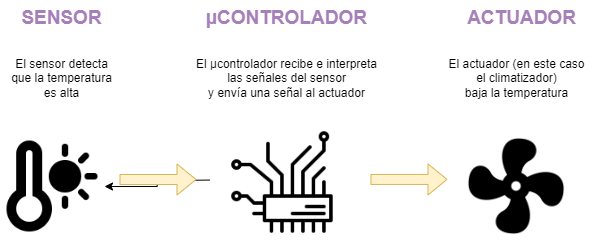
\includegraphics[width=0.70\textwidth]{imagenes/diagrama_sensor_actuador.png}
    \caption{Representación de sensores y actuadores. Elaboración propia}
\end{figure}

\subsubsection*{Sensores}

Los sensores tienen un papel esencial en el diseño hardware de las ECU, siendo los que proveen al microcontrolador de entradas para llevar a cabo operaciones y hacer funcionar el sistema. Normalmente un sensor de un vehículo da una medida de voltaje, que es representada por un código en el procesador. Si este voltaje es incorrecto, el micro lo tomará como una entrada inválida y dará un código de error. 

Existen decenas de sensores en un vehículo, pero aquí se van a citar algunos de los más relevantes [22]:


\begin{itemize}
    \item \textbf{Sensor Lambda: }También conocido como el sensor de oxígeno. Se encarga de medir la cantidad de oxígeno en los gases del escape para comprobar si las emisiones del vehículo están acorde al protocolo. 
    \item \textbf{Sensor de posición del acelerador (\textit{throttle})}: Este sensor permite determinar la posición del pedal del acelerador. Si está más presionado en vehículos de combustión, enviará más aire y combustible al motor. En el caso de los eléctricos, se enviará una señal para que se aumente el voltaje.
    \item \textbf{Sensor de líquido refrigerante: }El nombre es explicativo. Otorga los datos a la ECU para controlar si el nivel está bajo y necesita encenderse un testigo para comunicárselo al conductor.
    \item \textbf{Sensor de presión de los neumáticos}: Si bien no es algo común, el uso de estos sensores de presión en los tapones para las ruedas permite dar información al sistema sobre si la presión es correcta o existe alguna anomalía.
\end{itemize}

\subsubsection*{Actuadores}

Un actuador es un dispositivo eléctrico o mecánico que, al recibir una señal eléctrica enviada por el microcontrolador, la convierte a una acción mecánica. Son la contraparte directa de los sensores. Su funcionamiento depende del tipo de actuador y la energía que requiera, pero los pasos generales del proceso son los siguientes:

\begin{enumerate}
    \item 1. \textbf{Recepción de señal:} En primer lugar la ECU envía una señal al actuador, indicándole cuál es la acción que debe realizar. 
    \item 2. \textbf{Conversión señal-energía:} El actuador convierte la señal recibida al valor equivalente en la energía que precise, ya sea mecánica, neumática o hidráulica. 
    \item 3. \textbf{Activación:} El actuador realiza la acción acorde a los valores que ha recibido de la ECU, siendo algunos casos, por ejemplo, la activación del motor que baja las ventanas, el encendido de las luces de largo alcance, o cualquier otro mecanismo. 
    \item 4. \textbf{Feedback:} Mayormente en los casos más sensibles, el actuador envía a la ECU una señal indicando que su tarea ha sido realizada.
\end{enumerate}

\subsection{Interfaces de comunicación}
Con el aumento de sensores, actuadores y subsistemas en los vehículos, se ha hecho imperativo tener interconexión entre todas estas partes. En algunos casos, una conexión lenta o ineficiente puede conllevar un grave peligro, incluso vidas en riesgo. 

Para poder subsanar este problema se han desarrollado varios tipos de interfaces de comunicación, que permiten transmitir los datos de un subsistema al microcontrolador, o a otro subsistema. Dependiendo del contexto en el que se utilice, existen varios tipos de interfaces:

\begin{itemize}
    \item \textbf{CAN} \textit({Controller Area Network}): Sistema de buses de alta integridad para la interconexión de dispositivos inteligentes[23].  Está ampliamente extendida en la automoción, y funciona mediante una tecnología \textit{peer-to-peer} en la que no existe un maestro que controle el resto de nodos. Cada nodo CAN, una vez está listo para transmitir, comprueba si el bus está libre y escribe en la red. Tiene un sistema de prioridades dependiendo del nodo que envíe o reciba la señal. 
    \item \textbf{LIN} \textit({Local Interface Network}): Subsistema de la línea CAN. Se encarga de liberar la carga del bus que se genera al tener que supervisar la línea. Permite reducir costes y optimizar la comunicación.
    \item \textbf{FlexRay}: Esta interfaz actúa entre ECUs, y está destinada a aplicaciones críticas, como la ya nombrada anteriormente \textit{drive-by-wire}. Posee una alta transmisión de datos, redundacia y tolerancia de errores. Fue lanzada en 2007 en un BMW X5, y supuso un gran avance en la seguridad de los vehículos.
\end{itemize}

\section{La ECU en los vehículos: El mejor amigo del conductor}

El ser humano ha hecho grandes avances en la tecnología, y esto no podría ser menos en los vehículos. Las ECU que, como se ha visto en el apartado anteror, inicialmente no tenían tanta importancia, ahora se han convertido en algo fundamental para nosotros. Estas centralitas, que antiguamente servían únicamente para gestionar la inyección de combustible en el el motor, ahora tienen multitud de utilidades para cada una de las partes del vehículo.

Gracias a estos sistemas, podemos obtener desde una mayor eficiencia en el uso de la fuente de energía (ya sea combustible fósil o electricidad), un control más específico de los mapas motor para mayor potencia, recolección de datos relevantes del vehículo, e incluso algunas mejoras \textit{Quality of Life (QoL)} que nos permitan una conducción más cómoda. 

Muchos de estos sistemas no solamente inciden en la eficiencia y comodidad, sino también en la seguridad del conductor y de los pasajeros abordo. Algunas de las medidas más relevantes, que vamos a categorizar entre activas y pasivas, son las siguientes[11]:

\begin{enumerate}
    \item \textbf{Seguridad activa} - Conjunto de medidas que proporcionan mayor estabilidad al vehículo, buscando evitar el accidente a priori.
    \begin{itemize}
        \item \textit{Luces adaptativas}: Esta tecnología se basa en el uso de una matriz de LEDs en las luces delanteras, al contrario de la tradicional bombilla incandescente usada anteriormente. Los beneficios de este diseño son múltiples, pues permite modificar el haz de luz para evitar posibles deslumbramientos a otros usuarios de la vía, así como también adaptarse a las condiciones de la carretera, e iluminar más eficazmente el trazado.
     
        \item \textit{Control de crucero adaptativo (ACC)}: Permite mantener una velocidad designada por el conductor, variando cuando sea necesario por las condiciones del tráfico. Esta tecnología supone una gran ayuda en el caso de que exista una distracción del conductor. Puede funcionar junto a un sistema de detección de señales para no sobrepasar la velocidad máxima permitida en esa vía.
    
        \item \textit{Sistema de alerta de tráfico y evasión de colisión (TCAS)}: Este sistema tiene como tarea principal la detección de eventos en el tráfico que puedan causar un accidente, reaccionando (normalmente accionando de manera automática el freno), o advirtiendo al conductor para que sea él el que realice la acción pertinente para evitarlo.

        \item \textit{Sistema de detección de cansancio}: Algunos fabricantes [14] comienzan a implementar esta tecnología que, mediante sensores en la posición del conductor, o analizando su conducción, permite detectar si existen síntomas de cansancio o distracción. Normalmente muestran un aviso que se repite de manera continuada hasta que se realiza una parada. 
\end{itemize}

\begin{figure}[h]
    \centering
    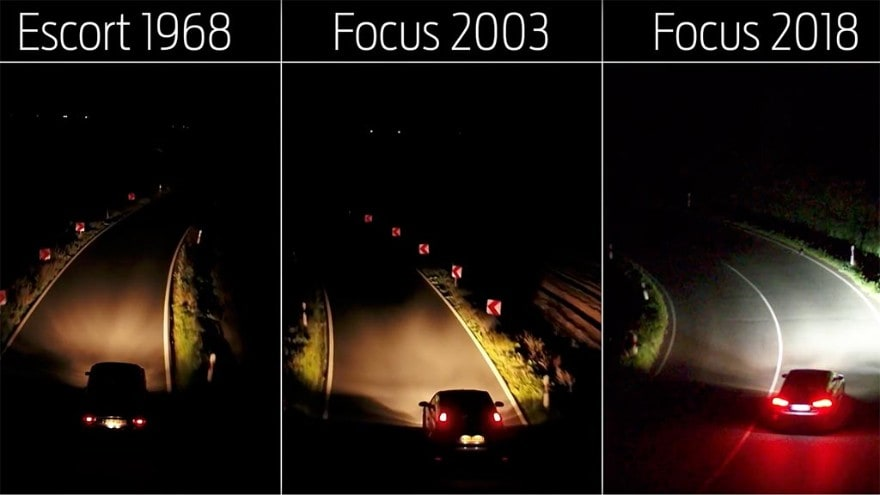
\includegraphics[width=0.7\textwidth]{imagenes/adaptive_lights.png}
    \caption{Comparación de la iluminación en los vehículos tras los años. Extraído de: [14]}
\end{figure}


    \item \textbf{Seguridad pasiva} - Conjunto de medidas que actúan una vez ha sucedido el accidente o el mal funcionamiento. Tienen el objetivo de minimizar los daños.

    \begin{itemize}
        \item \textit{Sistema de sensor de ocupación}: Permite detectar qué asientos están siendo utilizados, y comprobar el peso para saber si el ocupante es un niño o un adulto. Normalmente se utiliza para accionar el airbag si fuera necesario, y la altura a la que hacerlo.

        \item \textit{Notificación de colisión automática}: Este sistema envía un aviso a los servicios de emergencia de su localicación para que sea posible una intervención rápida.[16]
    \end{itemize}
\end{enumerate}




\section{La necesidad de un RTOS en las ECUs}

Como se ha mencionado en los apartados anteriores, los vehículos actuales poseen una gran multitud de sistemas y subsistemas que deben trabajar simultáneamente, teniendo unos márgenes temporales muy escasos y, en algunas situaciones, críticos para el funcionamiento del automóvil. 

Un sistema operativo que no fuera un RTOS podría causar desincronizaciones, respuestas demasiado lentas, y generar situaciones de peligro. 

Los RTOS permiten planificar, controlar y distribuir los núcleos de la CPU, para que todas esas funciones se realicen simultáneamente y en el tiempo de respuesta acotado, debido a su comportamiento determinista y predectible. 

Además, el uso de este tipo de SOs permite aislar los errores y prevenir que se extiendan al conjunto del vehículo, pues la planificación de los núcleos hace que sea posible mantener una tarea que monitorice los errores de manera continua y minimice el impacto de estos.
	% Estado del arte
	% 	1. Crítica al estado del arte
	% 	2. Propuesta	
	\chapter{Estudio de requisitos}

\fancyhead[R]{4. Estudio de requisitos}

\noindent\fbox{
	\parbox{\textwidth}{
        En este capítulo se sentarán las directrices del proyecto utilizando la ingeniería de requisitos. Esto servirá como base para la implementación del sistema, además de marcar los límites de este y las funcionalidades que se desarrollarán. 
    }

}


\section{Actores}
Lo primero que se debe hacer a la hora de diseñar un sistema es encontrar las entidades con las que este se comunica, llamadas \textbf{actores}. 
En este caso existen dos: el conductor, que controla el vehículo, y la ECU, que maneja los subsistemas. Desde un punto de vista formal, podemos describirlos así: 


\begin{table}[H]
    \begin{tabular}{|llllll|}
    \hline
    \multicolumn{1}{|l|}{\textbf{Actor}}           & \multicolumn{4}{l|}{Conductor}                                                                                                                                                  & AC-01                 \\ \hline
    \multicolumn{1}{|l|}{\textbf{Descripción}}     & \multicolumn{5}{l|}{Es el conductor del vehículo.}                                                                                                                                                      \\ \hline
    \multicolumn{1}{|l|}{\textbf{Características}} & \multicolumn{5}{l|}{\begin{tabular}[c]{@{}l@{}}Tiene que mantener su atención centrada en la carretera, por lo que no\\  debe distraerse demasiado con complicaciones en los subsistemas.\end{tabular}} \\ \hline
    \multicolumn{1}{|l|}{\textbf{Relaciones}}      & \multicolumn{5}{l|}{Necesita la ECU para poder controlar el vehículo.}                                                                                                                                  \\ \hline
    \multicolumn{1}{|l|}{\textbf{Referencias}}     & \multicolumn{5}{l|}{CU-01 .. CU-08}                                                                                                                                                                     \\ \hline
    \multicolumn{1}{|l|}{\textbf{Autor}}           & \multicolumn{1}{l|}{Sheila Martínez}        & \multicolumn{1}{l|}{\textbf{Fecha}}        & \multicolumn{1}{l|}{25/06/2023}        & \multicolumn{1}{l|}{\textbf{Versión}}       & 1.0                   \\ \hline
    \multicolumn{6}{|l|}{\cellcolor[HTML]{DAE8FC}\textbf{Atributos}}                                                                                                                                                                                         \\ \hline
    \multicolumn{1}{|l|}{\textbf{Nombre}}          & \multicolumn{4}{l|}{\textbf{Descripción}}                                                                                                                                       & \textbf{Tipo}         \\ \hline
    \multicolumn{1}{|l|}{Alias}                    & \multicolumn{4}{l|}{\begin{tabular}[c]{@{}l@{}}Nombre que introduce el conductor \\ para ser identificado en el vehículo\end{tabular}}                                          & cadena de texto       \\ \hline
    \end{tabular}
    \caption[Actor: Conductor]{Especificación del actor Conductor. Elaboración propia}
    \end{table}

\begin{table}[H]
    \begin{tabular}{|llllll|}
    \hline
    \multicolumn{1}{|l|}{\textbf{Actor}}           & \multicolumn{4}{l|}{ECU}                                                                                                                                                                      & AC-02                   \\ \hline
    \multicolumn{1}{|l|}{\textbf{Descripción}}     & \multicolumn{5}{l|}{Es la unidad de control del vehículo.}                                                                                                                                                              \\ \hline
    \multicolumn{1}{|l|}{\textbf{Características}} & \multicolumn{5}{l|}{\begin{tabular}[c]{@{}l@{}}Controla todos los subsistemas del vehículo. Siempre debe tener \\ información actualizada de los valores de los sensores, y actuar\\ cuando sea necesario\end{tabular}} \\ \hline
    \multicolumn{1}{|l|}{\textbf{Relaciones}}      & \multicolumn{5}{l|}{Es controlada indirectamente por el conductor del vehículo}                                                                                                                                         \\ \hline
    \multicolumn{1}{|l|}{\textbf{Referencias}}     & \multicolumn{5}{l|}{CU-01 .. CU-17}                                                                                                                                                                                     \\ \hline
    \multicolumn{1}{|l|}{\textbf{Autor}}           & \multicolumn{1}{l|}{Sheila Martínez}            & \multicolumn{1}{l|}{\textbf{Fecha}}           & \multicolumn{1}{l|}{25/06/2023}           & \multicolumn{1}{l|}{\textbf{Versión}}           & 1.0                     \\ \hline
    \multicolumn{6}{|l|}{\cellcolor[HTML]{DAE8FC}\textbf{Atributos}}                                                                                                                                                                                                         \\ \hline
    \multicolumn{1}{|l|}{\textbf{Nombre}}          & \multicolumn{4}{l|}{\textbf{Descripción}}                                                                                                                                                     & \textbf{Tipo}           \\ \hline
    \multicolumn{1}{|l|}{}                         & \multicolumn{4}{l|}{}                                                                                                                                                                         &                         \\ \hline
    \end{tabular}
    \caption[Actor: ECU]{Especificación del actor ECU. Elaboración propia}
    \end{table}



    
\section{Casos de Uso}


Antes de comenzar a desarrollar el sistema, y una vez hemos descrito los actores, debemos asegurarnos de cuáles serán sus funcionalidades y sus características. Comenzaremos generando casos de uso, es decir, acciones (incluyendo variantes y/o errores), que un sistema puede realizar al interactuar con los actores. 

\begin{table}[H]
    \resizebox{\textwidth}{!}{%
    \begin{tabular}{|l|l|l|l|l|l|}
    \hline
    \textbf{Caso de Uso} & \multicolumn{3}{l|}{Encender motor} & \multicolumn{2}{l|}{CU-01} \\ \hline
    \textbf{Actores} & \multicolumn{5}{l|}{Conductor (I), ECU} \\ \hline
    \textbf{Tipo} & \multicolumn{5}{l|}{Primario, Esencial} \\ \hline
    \textbf{Referencias} & RF1 & \multicolumn{4}{l|}{CU-10} \\ \hline
    \textbf{Precondición} & \multicolumn{5}{l|}{El motor debe estar apagado} \\ \hline
    \textbf{Postcondición} & \multicolumn{5}{l|}{El motor se habrá encendido} \\ \hline
    \textbf{Autor} & Sheila Martínez & \textbf{Fecha} & 23/06/2023 & \textbf{Versión} & v.1 \\ \hline
    \multicolumn{6}{|l|}{\cellcolor[HTML]{ECF4FF}Propósito} \\ \hline
    \multicolumn{6}{|l|}{El conductor pulsa un botón, la ECU enciende el motor} \\ \hline
    \multicolumn{6}{|l|}{\cellcolor[HTML]{ECF4FF}Resumen} \\ \hline
    \multicolumn{6}{|l|}{\begin{tabular}[c]{@{}l@{}}1. El conductor pulsa el botón de arranque.\\  2. La ECU comprueba que el motor está apagado. \\ 3. La ECU arranca el motor.\end{tabular}} \\ \hline
    \end{tabular}%
    }
    \end{table}

    
\begin{table}[H]
    \resizebox{\textwidth}{!}{%
    \begin{tabular}{|l|l|l|l|l|l|}
    \hline
    \textbf{Caso de Uso} & \multicolumn{3}{l|}{Apagar motor} & \multicolumn{2}{l|}{CU-02} \\ \hline
    \textbf{Actores} & \multicolumn{5}{l|}{Conductor (I), ECU} \\ \hline
    \textbf{Tipo} & \multicolumn{5}{l|}{Primario, Esencial} \\ \hline
    \textbf{Referencias} & RF2 & \multicolumn{4}{l|}{CU-10} \\ \hline
    \textbf{Precondición} & \multicolumn{5}{l|}{El motor debe estar encendido} \\ \hline
    \textbf{Postcondición} & \multicolumn{5}{l|}{El motor se habrá apagado} \\ \hline
    \textbf{Autor} & Sheila Martínez & \textbf{Fecha} & 23/06/2023 & \textbf{Versión} & v.1 \\ \hline
    \multicolumn{6}{|l|}{\cellcolor[HTML]{ECF4FF}Propósito} \\ \hline
    \multicolumn{6}{|l|}{El conductor pulsa un botón, la ECU apaga el motor} \\ \hline
    \multicolumn{6}{|l|}{\cellcolor[HTML]{ECF4FF}Resumen} \\ \hline
    \multicolumn{6}{|l|}{\begin{tabular}[c]{@{}l@{}}1. El conductor pulsa el botón de apagado.\\  2. La ECU comprueba que el motor está encendido. \\ 3. La ECU apaga el motor.\end{tabular}} \\ \hline
    \end{tabular}%
    }
    \end{table}    


\begin{table}[H]
    \resizebox{\textwidth}{!}{%
    \begin{tabular}{|l|l|l|l|l|l|}
    \hline
    \textbf{Caso de Uso} & \multicolumn{3}{l|}{Encender luces} & \multicolumn{2}{l|}{CU-03} \\ \hline
    \textbf{Actores} & \multicolumn{5}{l|}{Conductor (I), ECU} \\ \hline
    \textbf{Tipo} & \multicolumn{5}{l|}{Primario, Esencial} \\ \hline
    \textbf{Referencias} & RF3 & \multicolumn{4}{l|}{CU-11} \\ \hline
    \textbf{Precondición} & \multicolumn{5}{l|}{Las luces deben estar apagadas} \\ \hline
    \textbf{Postcondición} & \multicolumn{5}{l|}{Las luces se habrán encendido} \\ \hline
    \textbf{Autor} & Sheila Martínez & \textbf{Fecha} & 23/06/2023 & \textbf{Versión} & v.1 \\ \hline
    \multicolumn{6}{|l|}{\cellcolor[HTML]{ECF4FF}Propósito} \\ \hline
    \multicolumn{6}{|l|}{El conductor pulsa un botón, la ECU enciende las luces} \\ \hline
    \multicolumn{6}{|l|}{\cellcolor[HTML]{ECF4FF}Resumen} \\ \hline
    \multicolumn{6}{|l|}{\begin{tabular}[c]{@{}l@{}}1. El conductor pulsa el botón de encendido de luces.\\  2. La ECU comprueba que las luces están apagadas. \\ 3. La ECU enciende las luces \\ 4. La ECU enciende el piloto que indica que las luces están encendidas.\end{tabular}} \\ \hline
    \end{tabular}%
    }
\end{table}


\begin{table}[H]
    \resizebox{\textwidth}{!}{%
    \begin{tabular}{|l|l|l|l|l|l|}
    \hline
    \textbf{Caso de Uso} & \multicolumn{3}{l|}{Apagar luces} & \multicolumn{2}{l|}{CU-04} \\ \hline
    \textbf{Actores} & \multicolumn{5}{l|}{Conductor (I), ECU} \\ \hline
    \textbf{Tipo} & \multicolumn{5}{l|}{Primario, Esencial} \\ \hline
    \textbf{Referencias} & RF3 & \multicolumn{4}{l|}{CU-11} \\ \hline
    \textbf{Precondición} & \multicolumn{5}{l|}{Las luces deben estar encendidas} \\ \hline
    \textbf{Postcondición} & \multicolumn{5}{l|}{Las luces se habrán apagado} \\ \hline
    \textbf{Autor} & Sheila Martínez & \textbf{Fecha} & 23/06/2023 & \textbf{Versión} & v.1 \\ \hline
    \multicolumn{6}{|l|}{\cellcolor[HTML]{ECF4FF}Propósito} \\ \hline
    \multicolumn{6}{|l|}{El conductor pulsa un botón, la ECU apaga las luces} \\ \hline
    \multicolumn{6}{|l|}{\cellcolor[HTML]{ECF4FF}Resumen} \\ \hline
    \multicolumn{6}{|l|}{\begin{tabular}[c]{@{}l@{}}1. El conductor pulsa el botón de apagado de luces.\\ 2. La ECU comprueba que las luces están encendidas.\\ 3. La ECU apaga las luces.\end{tabular}} \\ \hline
    \end{tabular}%
    }
    \end{table}

\begin{table}[H]
    \resizebox{\textwidth}{!}{%
    \begin{tabular}{|l|l|l|l|l|l|}
    \hline
    \textbf{Caso de Uso} & \multicolumn{3}{l|}{Encender intermitente} & \multicolumn{2}{l|}{CU-05} \\ \hline
    \textbf{Actores} & \multicolumn{5}{l|}{Conductor (I), ECU} \\ \hline
    \textbf{Tipo} & \multicolumn{5}{l|}{Primario, Esencial} \\ \hline
    \textbf{Referencias} & RF5 & \multicolumn{4}{l|}{CU-11} \\ \hline
    \textbf{Precondición} & \multicolumn{5}{l|}{Los intermitentes deben estar apagados} \\ \hline
    \textbf{Postcondición} & \multicolumn{5}{l|}{Se habrá accionado el intermitente de la dirección deseada} \\ \hline
    \textbf{Autor} & Sheila Martínez & \textbf{Fecha} & 23/06/2023 & \textbf{Versión} & v.1 \\ \hline
    \multicolumn{6}{|l|}{\cellcolor[HTML]{ECF4FF}Propósito} \\ \hline
    \multicolumn{6}{|l|}{El conductor acciona una palanca, la ECU enciende la luz intermitente} \\ \hline
    \multicolumn{6}{|l|}{\cellcolor[HTML]{ECF4FF}Resumen} \\ \hline
    \multicolumn{6}{|l|}{\begin{tabular}[c]{@{}l@{}}1. El conductor acciona la palanca hacia el lado deseado\\ 2. La ECU comprueba que el intermitente no está accionado\\ 3. La ECU enciende el intermitente de ese lado\end{tabular}} \\ \hline
    \end{tabular}%
    }
    \end{table}

\begin{table}[H]
    \resizebox{\textwidth}{!}{%
    \begin{tabular}{|l|l|l|l|l|l|}
    \hline
    \textbf{Caso de Uso} & \multicolumn{3}{l|}{Apagar intermitente} & \multicolumn{2}{l|}{CU-06} \\ \hline
    \textbf{Actores} & \multicolumn{5}{l|}{Conductor (I), ECU} \\ \hline
    \textbf{Tipo} & \multicolumn{5}{l|}{Primario, Esencial} \\ \hline
    \textbf{Referencias} & RF6 & \multicolumn{4}{l|}{CU-11} \\ \hline
    \textbf{Precondición} & \multicolumn{5}{l|}{El intermitente debe estar accionado hacia uno de los dos lados} \\ \hline
    \textbf{Postcondición} & \multicolumn{5}{l|}{Se habrán apagado los intermitentes} \\ \hline
    \textbf{Autor} & Sheila Martínez & \textbf{Fecha} & 23/06/2023 & \textbf{Versión} & v.1 \\ \hline
    \multicolumn{6}{|l|}{\cellcolor[HTML]{ECF4FF}Propósito} \\ \hline
    \multicolumn{6}{|l|}{El conductor devuelve una palanca a su estado inicial, la ECU apaga la luz intermitente} \\ \hline
    \multicolumn{6}{|l|}{\cellcolor[HTML]{ECF4FF}Resumen} \\ \hline
    \multicolumn{6}{|l|}{\begin{tabular}[c]{@{}l@{}}1. El conductor devuelve la palanca hacia su estado inicial\\ 2. La ECU apaga los intermitentes\end{tabular}} \\ \hline
    \end{tabular}%
    }
\end{table}

\begin{table}[H]
    \resizebox{\textwidth}{!}{%
    \begin{tabular}{|l|l|l|l|l|l|}
    \hline
    \textbf{Caso de Uso} & \multicolumn{3}{l|}{Cambiar estado luz freno} & \multicolumn{2}{l|}{CU-07} \\ \hline
    \textbf{Actores} & \multicolumn{5}{l|}{Conductor (I), ECU} \\ \hline
    \textbf{Tipo} & \multicolumn{5}{l|}{Primario, Esencial} \\ \hline
    \textbf{Referencias} & RF7 & \multicolumn{4}{l|}{CU-11} \\ \hline
    \textbf{Precondición} & \multicolumn{5}{l|}{} \\ \hline
    \textbf{Postcondición} & \multicolumn{5}{l|}{Se habrá encendido la luz de freno} \\ \hline
    \textbf{Autor} & Sheila Martínez & \textbf{Fecha} & 23/06/2023 & \textbf{Versión} & v.1 \\ \hline
    \multicolumn{6}{|l|}{\cellcolor[HTML]{ECF4FF}Propósito} \\ \hline
    \multicolumn{6}{|l|}{El conductor pisa el pedal de freno, se enciende la luz de freno} \\ \hline
    \multicolumn{6}{|l|}{\cellcolor[HTML]{ECF4FF}Resumen} \\ \hline
    \multicolumn{6}{|l|}{\begin{tabular}[c]{@{}l@{}}1. El conductor pisa el pedal de freno\\ 2. La ECU detecta que el freno ha sido pulsado\\ 3. La ECU enciende la luz de freno\\ 3.1 El conductor suelta el pedal de freno\\ 3.2 La ECU detecta que el freno ha sido soltado\\ 3.3 La ECU apaga la luz de freno\end{tabular}} \\ \hline
    \end{tabular}%
    }
\end{table}


\begin{table}[H]
    \resizebox{\textwidth}{!}{%
    \begin{tabular}{|l|l|l|l|l|l|}
    \hline
    \textbf{Caso de Uso} & \multicolumn{3}{l|}{Cambiar velocidad} & \multicolumn{2}{l|}{CU-08} \\ \hline
    \textbf{Actores} & \multicolumn{5}{l|}{Conductor (I), ECU} \\ \hline
    \textbf{Tipo} & \multicolumn{5}{l|}{Primario, Esencial} \\ \hline
    \textbf{Referencias} & RF8 & \multicolumn{4}{l|}{-} \\ \hline
    \textbf{Precondición} & \multicolumn{5}{l|}{El motor debe estar encendido} \\ \hline
    \textbf{Postcondición} & \multicolumn{5}{l|}{Se habrá variado la velocidad} \\ \hline
    \textbf{Autor} & Sheila Martínez & \textbf{Fecha} & 23/06/2023 & \textbf{Versión} & v.1 \\ \hline
    \multicolumn{6}{|l|}{\cellcolor[HTML]{ECF4FF}Propósito} \\ \hline
    \multicolumn{6}{|l|}{El conductor pisa el pedal de acelerador, el motor acelera proporcionalmente} \\ \hline
    \multicolumn{6}{|l|}{\cellcolor[HTML]{ECF4FF}Resumen} \\ \hline
    \multicolumn{6}{|l|}{\begin{tabular}[c]{@{}l@{}}1. El conductor pisa el acelerador\\ 2. La ECU detecta que ha sido pulsado y con cuánta intensidad.\\ 3. La ECU varía la velocidad en función de la intensidad.\end{tabular}} \\ \hline
    \end{tabular}%
    }
    \end{table}


\begin{table}[H]
    \resizebox{\textwidth}{!}{%
    \begin{tabular}{|l|l|l|l|l|l|}
    \hline
    \textbf{Caso de Uso} & \multicolumn{3}{l|}{Comprobar temperatura motor} & \multicolumn{2}{l|}{CU-09} \\ \hline
    \textbf{Actores} & \multicolumn{5}{l|}{ECU} \\ \hline
    \textbf{Tipo} & \multicolumn{5}{l|}{Primario, Esencial} \\ \hline
    \textbf{Referencias} & RF9 & \multicolumn{4}{l|}{CU-17} \\ \hline
    \textbf{Precondición} & \multicolumn{5}{l|}{} \\ \hline
    \textbf{Postcondición} & \multicolumn{5}{l|}{Se habrá leído y comprobado el valor de la temperatura del motor} \\ \hline
    \textbf{Autor} & Sheila Martínez & \textbf{Fecha} & 23/06/2023 & \textbf{Versión} & v.1 \\ \hline
    \multicolumn{6}{|l|}{\cellcolor[HTML]{ECF4FF}Propósito} \\ \hline
    \multicolumn{6}{|l|}{La ECU obtiene el valor de la temperatura del motor y comprueba si es correcta.} \\ \hline
    \multicolumn{6}{|l|}{\cellcolor[HTML]{ECF4FF}Resumen} \\ \hline
    \multicolumn{6}{|l|}{\begin{tabular}[c]{@{}l@{}}1. La ECU obtiene el valor de la temperatura del motor.\\ 2. Comprueba si el valor es correcto.\\ \\ 2.1 Si es incorrecto, enciende un piloto que lo indica.\end{tabular}} \\ \hline
    \end{tabular}%
    }
    \end{table}

    \begin{table}[H]
        \resizebox{\textwidth}{!}{%
        \begin{tabular}{|l|l|l|l|l|l|}
        \hline
        \textbf{Caso de Uso} & \multicolumn{3}{l|}{Comprobar estado motor} & \multicolumn{2}{l|}{CU-10} \\ \hline
        \textbf{Actores} & \multicolumn{5}{l|}{ECU} \\ \hline
        \textbf{Tipo} & \multicolumn{5}{l|}{Primario, Esencial} \\ \hline
        \textbf{Referencias} & RF9 & \multicolumn{4}{l|}{-} \\ \hline
        \textbf{Precondición} & \multicolumn{5}{l|}{} \\ \hline
        \textbf{Postcondición} & \multicolumn{5}{l|}{Se habrá leído y comprobado el estado del motor} \\ \hline
        \textbf{Autor} & Sheila Martínez & \textbf{Fecha} & 23/06/2023 & \textbf{Versión} & v.1 \\ \hline
        \multicolumn{6}{|l|}{\cellcolor[HTML]{ECF4FF}Propósito} \\ \hline
        \multicolumn{6}{|l|}{La ECU obtiene el estado del motor} \\ \hline
        \multicolumn{6}{|l|}{\cellcolor[HTML]{ECF4FF}Resumen} \\ \hline
        \multicolumn{6}{|l|}{\begin{tabular}[c]{@{}l@{}}1. La ECU obtiene el estado del motor \end{tabular}} \\ \hline
        \end{tabular}%
        }
        \end{table}


\begin{table}[H]
    \resizebox{\textwidth}{!}{%
    \begin{tabular}{|l|l|l|l|l|l|}
    \hline
    \textbf{Caso de Uso} & \multicolumn{3}{l|}{Comprobar estado luces} & \multicolumn{2}{l|}{CU-11} \\ \hline
    \textbf{Actores} & \multicolumn{5}{l|}{ECU} \\ \hline
    \textbf{Tipo} & \multicolumn{5}{l|}{Primario, Esencial} \\ \hline
    \textbf{Referencias} & RF9 & \multicolumn{4}{l|}{-} \\ \hline
    \textbf{Precondición} & \multicolumn{5}{l|}{} \\ \hline
    \textbf{Postcondición} & \multicolumn{5}{l|}{Se habrá leído y comprobado el estado de las luces} \\ \hline
    \textbf{Autor} & Sheila Martínez & \textbf{Fecha} & 23/06/2023 & \textbf{Versión} & v.1 \\ \hline
    \multicolumn{6}{|l|}{\cellcolor[HTML]{ECF4FF}Propósito} \\ \hline
    \multicolumn{6}{|l|}{La ECU obtiene el estado de las luces} \\ \hline
    \multicolumn{6}{|l|}{\cellcolor[HTML]{ECF4FF}Resumen} \\ \hline
    \multicolumn{6}{|l|}{1. La ECU obtiene el estado de las luces} \\ \hline
    \end{tabular}%
    }
    \end{table}


    \begin{table}[H]
        \resizebox{\textwidth}{!}{%
        \begin{tabular}{|l|l|l|l|l|l|}
        \hline
        \textbf{Caso de Uso} & \multicolumn{3}{l|}{Comprobar temperatura batería} & \multicolumn{2}{l|}{CU-12} \\ \hline
        \textbf{Actores} & \multicolumn{5}{l|}{ECU} \\ \hline
        \textbf{Tipo} & \multicolumn{5}{l|}{Primario, Esencial} \\ \hline
        \textbf{Referencias} & RF9 & \multicolumn{4}{l|}{CU-17} \\ \hline
        \textbf{Precondición} & \multicolumn{5}{l|}{} \\ \hline
        \textbf{Postcondición} & \multicolumn{5}{l|}{Se habrá leído y comprobado el valor de la temperatura de la batería} \\ \hline
        \textbf{Autor} & Sheila Martínez & \textbf{Fecha} & 23/06/2023 & \textbf{Versión} & v.1 \\ \hline
        \multicolumn{6}{|l|}{\cellcolor[HTML]{ECF4FF}Propósito} \\ \hline
        \multicolumn{6}{|l|}{La ECU obtiene el valor de la temperatura de la batería y comprueba si es correcta.} \\ \hline
        \multicolumn{6}{|l|}{\cellcolor[HTML]{ECF4FF}Resumen} \\ \hline
        \multicolumn{6}{|l|}{\begin{tabular}[c]{@{}l@{}}1. La ECU obtiene el valor de la temperatura de la batería.\\ 2. Comprueba si el valor es correcto.\\ \\ 2.1 Si es incorrecto, enciende un piloto que lo indica.\end{tabular}} \\ \hline
        \end{tabular}%
        }
        \end{table}


        \begin{table}[H]
            \resizebox{\textwidth}{!}{%
            \begin{tabular}{|l|l|l|l|l|l|}
            \hline
            \textbf{Caso de Uso} & \multicolumn{3}{l|}{Leer voltaje sistema} & \multicolumn{2}{l|}{CU-13} \\ \hline
            \textbf{Actores} & \multicolumn{5}{l|}{ECU} \\ \hline
            \textbf{Tipo} & \multicolumn{5}{l|}{Primario, Real} \\ \hline
            \textbf{Referencias} & RF9 & \multicolumn{4}{l|}{-} \\ \hline
            \textbf{Precondición} & \multicolumn{5}{l|}{} \\ \hline
            \textbf{Postcondición} & \multicolumn{5}{l|}{Se habrá leído y comprobado el voltaje} \\ \hline
            \textbf{Autor} & Sheila Martínez & \textbf{Fecha} & 23/06/2023 & \textbf{Versión} & v.1 \\ \hline
            \multicolumn{6}{|l|}{\cellcolor[HTML]{ECF4FF}Propósito} \\ \hline
            \multicolumn{6}{|l|}{La ECU obtiene el voltaje del sistema} \\ \hline
            \multicolumn{6}{|l|}{\cellcolor[HTML]{ECF4FF}Resumen} \\ \hline
            \multicolumn{6}{|l|}{1. La ECU obtiene el voltaje del sistema} \\ \hline
            \end{tabular}%
            }
            \end{table}


\begin{table}[H]
    \resizebox{\textwidth}{!}{%
    \begin{tabular}{|l|l|l|l|l|l|}
    \hline
    \textbf{Caso de Uso} & \multicolumn{3}{l|}{Calcular consumo} & \multicolumn{2}{l|}{CU-14} \\ \hline
    \textbf{Actores} & \multicolumn{5}{l|}{ECU} \\ \hline
    \textbf{Tipo} & \multicolumn{5}{l|}{Primario, Esencial} \\ \hline
    \textbf{Referencias} & RF9 & \multicolumn{4}{l|}{CU-13} \\ \hline
    \textbf{Precondición} & \multicolumn{5}{l|}{Se debe haber leído el voltaje de la batería} \\ \hline
    \textbf{Postcondición} & \multicolumn{5}{l|}{Se habrá calculado el consumo} \\ \hline
    \textbf{Autor} & Sheila Martínez & \textbf{Fecha} & 23/06/2023 & \textbf{Versión} & v.1 \\ \hline
    \multicolumn{6}{|l|}{\cellcolor[HTML]{ECF4FF}Propósito} \\ \hline
    \multicolumn{6}{|l|}{La ECU obtiene el consumo instantáneo} \\ \hline
    \multicolumn{6}{|l|}{\cellcolor[HTML]{ECF4FF}Resumen} \\ \hline
    \multicolumn{6}{|l|}{1. La ECU obtiene el consumo instantáneo} \\ \hline
    \end{tabular}%
    }
    \end{table}

\begin{table}[H]
    \resizebox{\textwidth}{!}{%
    \begin{tabular}{|l|l|l|l|l|l|}
    \hline
    \textbf{Caso de Uso} & \multicolumn{3}{l|}{Calcular autonomía} & \multicolumn{2}{l|}{CU-15} \\ \hline
    \textbf{Actores} & \multicolumn{5}{l|}{ECU} \\ \hline
    \textbf{Tipo} & \multicolumn{5}{l|}{Primario, Esencial} \\ \hline
    \textbf{Referencias} & RF9 & \multicolumn{4}{l|}{CU-14} \\ \hline
    \textbf{Precondición} & \multicolumn{5}{l|}{Se debe saber el voltaje máximo de la batería y el consumo} \\ \hline
    \textbf{Postcondición} & \multicolumn{5}{l|}{Se habrá calculado la autonomía} \\ \hline
    \textbf{Autor} & Sheila Martínez & \textbf{Fecha} & 23/06/2023 & \textbf{Versión} & v.1 \\ \hline
    \multicolumn{6}{|l|}{\cellcolor[HTML]{ECF4FF}Propósito} \\ \hline
    \multicolumn{6}{|l|}{La ECU obtiene la autonomía del sistema} \\ \hline
    \multicolumn{6}{|l|}{\cellcolor[HTML]{ECF4FF}Resumen} \\ \hline
    \multicolumn{6}{|l|}{La ECU obtiene la autonomía del sistema en tiempo y porcentaje} \\ \hline
    \end{tabular}%
    }
    \end{table}


\begin{table}[H]
    \resizebox{\textwidth}{!}{%
    \begin{tabular}{|l|l|l|l|l|l|}
    \hline
    \textbf{Caso de Uso} & \multicolumn{3}{l|}{Calcular carga batería} & \multicolumn{2}{l|}{CU-16} \\ \hline
    \textbf{Actores} & \multicolumn{5}{l|}{ECU} \\ \hline
    \textbf{Tipo} & \multicolumn{5}{l|}{Primario, Esencial} \\ \hline
    \textbf{Referencias} & RF9 & \multicolumn{4}{l|}{CU-13} \\ \hline
    \textbf{Precondición} & \multicolumn{5}{l|}{Se debe saber el voltaje máximo de la batería y el voltaje actual} \\ \hline
    \textbf{Postcondición} & \multicolumn{5}{l|}{Se habrá calculado la carga de la batería} \\ \hline
    \textbf{Autor} & Sheila Martínez & \textbf{Fecha} & 23/06/2023 & \textbf{Versión} & v.1 \\ \hline
    \multicolumn{6}{|l|}{\cellcolor[HTML]{ECF4FF}Propósito} \\ \hline
    \multicolumn{6}{|l|}{La ECU obtiene la carga de la batería} \\ \hline
    \multicolumn{6}{|l|}{\cellcolor[HTML]{ECF4FF}Resumen} \\ \hline
    \multicolumn{6}{|l|}{La ECU obtiene la carga de la batería en porcentaje} \\ \hline
    \end{tabular}%
    }
    \end{table}

\begin{table}[H]
    \resizebox{\textwidth}{!}{%
    \begin{tabular}{|l|l|l|l|l|l|}
    \hline
    \textbf{Caso de Uso} & \multicolumn{3}{l|}{Mostrar datos} & \multicolumn{2}{l|}{CU-17} \\ \hline
    \textbf{Actores} & \multicolumn{5}{l|}{ECU} \\ \hline
    \textbf{Tipo} & \multicolumn{5}{l|}{Primario, Esencial} \\ \hline
    \textbf{Referencias} & RF9 & \multicolumn{4}{l|}{-} \\ \hline
    \textbf{Precondición} & \multicolumn{5}{l|}{Se deben tener calculados y leídos todos los datos del sistema} \\ \hline
    \textbf{Postcondición} & \multicolumn{5}{l|}{Se mostrarán los datos del sistema} \\ \hline
    \textbf{Autor} & Sheila Martínez & \textbf{Fecha} & 23/06/2023 & \textbf{Versión} & v.1 \\ \hline
    \multicolumn{6}{|l|}{\cellcolor[HTML]{ECF4FF}Propósito} \\ \hline
    \multicolumn{6}{|l|}{La ECU muestra los datos del sistema} \\ \hline
    \multicolumn{6}{|l|}{\cellcolor[HTML]{ECF4FF}Resumen} \\ \hline
    \multicolumn{6}{|l|}{\begin{tabular}[c]{@{}l@{}}La ECU muestra por pantalla todos los datos obtenidos por los sensores\\  para que el conductor pueda servirse de ellos\end{tabular}} \\ \hline
    \end{tabular}%
    }
\end{table}

\newpage
\section{Diagramas de casos de uso}

Una vez realizados los casos de uso, los \textbf{diagramas de uso} nos permiten tener una visión general del conjunto de subsistemas, así como su interacción con los actores: 


\begin{figure}[H]
    \centering
    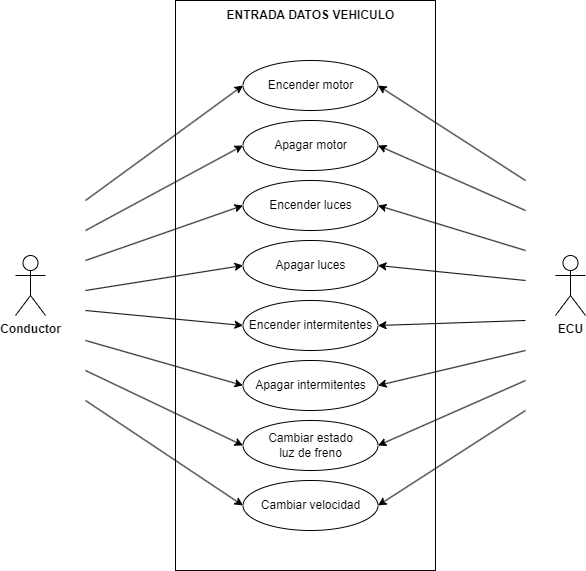
\includegraphics[width=1.1\textwidth]{imagenes/diagrama_CU_1.png}
\end{figure}

\begin{figure}[H]
    \centering
    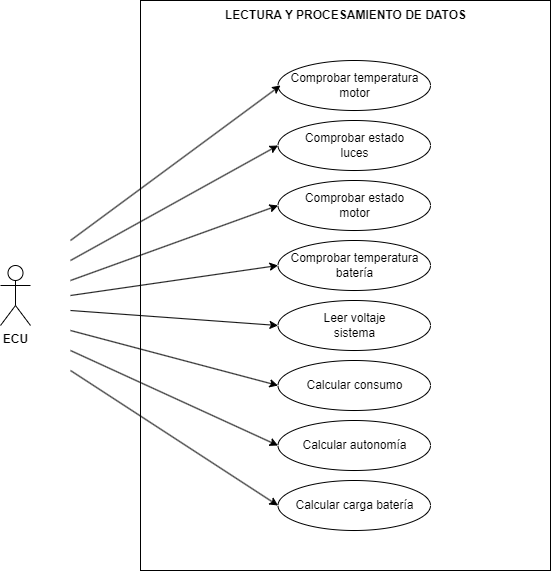
\includegraphics[width=1\textwidth]{imagenes/diagrama_CU_2.png}
\end{figure}

\begin{figure}[H]
    \centering
    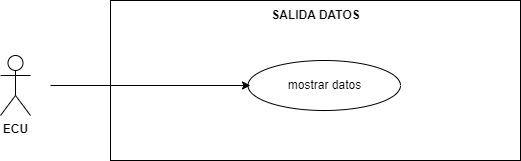
\includegraphics[width=1\textwidth]{imagenes/diagrama_CU_3.png}
\end{figure}


\section{Requisitos}

Los requisitos nos van a permitir comprender y designar cuáles serán las capacidades y funciones de nuestro producto para resolver una necesidad expresada por el usuario. Existen dos tipos principales, que se exponen a continuación.

\subsection{Requisitos funcionales}

Los requisitos funcionales son aquellos requisitos que describen las funciones que debe realizar el sistema, es decir, la interacción entre este y su entorno, e indican cuál debe ser la reacción al sistema ante una determinada entrada. 

\begin{table}[H]
    \resizebox{\textwidth}{!}{%
    \begin{tabular}{|l|l|}
    \hline
    \textbf{Nº de RF} & 1 \\ \hline
    \textbf{Nombre} & Encender el motor \\ \hline
    \textbf{Descripción} & Como conductor, quiero poder encender el motor del vehículo \\ \hline
    \textbf{Prioridad} & Alta \\ \hline
    \textbf{Entrada} & Una señal \\ \hline
    \textbf{Prerrequisitos} & El motor debe estar apagado \\ \hline
    \textbf{Procesamiento} & El usuario pulsa el botón de arranque y el motor se activa \\ \hline
    \rowcolor[HTML]{FFFFFF} 
    \textbf{Postcondición} & - \\ \hline
    \end{tabular}%
    }
    \end{table}

\begin{table}[H]
    \resizebox{\textwidth}{!}{%
    \begin{tabular}{|l|l|}
    \hline
    \textbf{Nº de RF} & 2 \\ \hline
    \textbf{Nombre} & Apagar el motor \\ \hline
    \textbf{Descripción} & Como conductor, quiero poder apagar el motor del vehículo \\ \hline
    \textbf{Prioridad} & Alta \\ \hline
    \textbf{Entrada} & Una señal \\ \hline
    \textbf{Prerrequisitos} & El motor debe estar encendido \\ \hline
    \textbf{Procesamiento} & El usuario pulsa el botón de arranque y el motor se apaga \\ \hline
    \rowcolor[HTML]{FFFFFF} 
    \textbf{Postcondición} & - \\ \hline
    \end{tabular}%
    }
    \end{table}


\begin{table}[H]
    \resizebox{\textwidth}{!}{%
    \begin{tabular}{|l|l|}
    \hline
    \textbf{Nº de RF} & 3 \\ \hline
    \textbf{Nombre} & Encender las luces \\ \hline
    \textbf{Descripción} & Como conductor, quiero poder encender las luces del vehículo \\ \hline
    \textbf{Prioridad} & Media \\ \hline
    \textbf{Entrada} & Una señal \\ \hline
    \textbf{Prerrequisitos} & Las luces deben estar apagadas \\ \hline
    \textbf{Procesamiento} & El usuario pulsa el botón de encendido de luces y las luces se encienden \\ \hline
    \rowcolor[HTML]{FFFFFF} 
    \textbf{Postcondición} & - \\ \hline
    \end{tabular}%
    }
    \end{table}


\begin{table}[H]
    \resizebox{\textwidth}{!}{%
    \begin{tabular}{|l|l|}
    \hline
    \textbf{Nº de RF} & 4 \\ \hline
    \textbf{Nombre} & Apagar las luces \\ \hline
    \textbf{Descripción} & Como conductor, quiero poder apagar las luces del vehículo \\ \hline
    \textbf{Prioridad} & Media \\ \hline
    \textbf{Entrada} & Una señal \\ \hline
    \textbf{Prerrequisitos} & Las luces deben estar encendidas \\ \hline
    \textbf{Procesamiento} & El usuario pulsa el botón de apagado de luces y las luces se apagan \\ \hline
    \rowcolor[HTML]{FFFFFF} 
    \textbf{Postcondición} & - \\ \hline
    \end{tabular}%
    }
    \end{table}

\begin{table}[H]
    \resizebox{\textwidth}{!}{%
    \begin{tabular}{|l|l|}
    \hline
    \textbf{Nº de RF} & 5 \\ \hline
    \textbf{Nombre} & Encender intermitentes \\ \hline
    \textbf{Descripción} & Como conductor, quiero poder encender el intermitente de un lado del vehículo \\ \hline
    \textbf{Prioridad} & Media \\ \hline
    \textbf{Entrada} & Una señal \\ \hline
    \textbf{Prerrequisitos} & El intermitente debe estar en su posición inicial (apagado) \\ \hline
    \textbf{Procesamiento} & \begin{tabular}[c]{@{}l@{}}El usuario mueve la palanca hacia el lado determinado y el intermitente de ese\\ lado se enciende\end{tabular} \\ \hline
    \rowcolor[HTML]{FFFFFF} 
    \textbf{Postcondición} & - \\ \hline
    \end{tabular}%
    }
    \end{table}

\begin{table}[H]
    \resizebox{\textwidth}{!}{%
    \begin{tabular}{|l|l|}
    \hline
    \textbf{Nº de RF} & 6 \\ \hline
    \textbf{Nombre} & Apagar intermitentes \\ \hline
    \textbf{Descripción} & Como conductor, quiero poder apagar el intermitente de un lado del vehículo \\ \hline
    \textbf{Prioridad} & Media \\ \hline
    \textbf{Entrada} & Una señal \\ \hline
    \textbf{Prerrequisitos} & El intermitente no debe estar en su posición inicial (debe estar encendido) \\ \hline
    \textbf{Procesamiento} & El usuario mueve la palanca hacia su posición inicial y los intermitentes se apagan \\ \hline
    \rowcolor[HTML]{FFFFFF} 
    \textbf{Postcondición} & - \\ \hline
    \end{tabular}%
    }
    \end{table}

\begin{table}[H]
    \resizebox{\textwidth}{!}{%
    \begin{tabular}{|l|l|}
    \hline
    \textbf{Nº de RF} & 7 \\ \hline
    \textbf{Nombre} & Cambiar estado de la luz de freno \\ \hline
    \textbf{Descripción} & Como conductor, quiero poder pisar el freno y que se encienda la luz correspondiente \\ \hline
    \textbf{Prioridad} & Alta \\ \hline
    \textbf{Entrada} & Una señal \\ \hline
    \textbf{Prerrequisitos} & - \\ \hline
    \textbf{Procesamiento} & \begin{tabular}[c]{@{}l@{}}La luz de freno se enciende cuando el conductor pisa el freno, y se apaga cuando\\ deja de pulsarlo\end{tabular} \\ \hline
    \rowcolor[HTML]{FFFFFF} 
    \textbf{Postcondición} & - \\ \hline
    \end{tabular}%
    }
    \end{table}

\begin{table}[H]
    \resizebox{\textwidth}{!}{%
    \begin{tabular}{|l|l|}
    \hline
    \textbf{Nº de RF} & 8 \\ \hline
    \textbf{Nombre} & Cambiar velocidad \\ \hline
    \textbf{Descripción} & Como conductor, quiero poder pisar el acelerador  y que el motor acelere \\ \hline
    \textbf{Prioridad} & Alta \\ \hline
    \textbf{Entrada} & Una señal \\ \hline
    \textbf{Prerrequisitos} & - \\ \hline
    \textbf{Procesamiento} & \begin{tabular}[c]{@{}l@{}}El motor aumenta su velocidad proporcionalmente al recorrido que haya \\ hecho el pedal de acelerador al ser pisado por el conductor\end{tabular} \\ \hline
    \rowcolor[HTML]{FFFFFF} 
    \textbf{Postcondición} & - \\ \hline
    \end{tabular}%
    }
    \end{table}

\begin{table}[H]
    \resizebox{\textwidth}{!}{%
    \begin{tabular}{|l|l|}
    \hline
    \textbf{Nº de RF} & 9 \\ \hline
    \textbf{Nombre} & Comprobar datos del sistema \\ \hline
    \textbf{Descripción} & \begin{tabular}[c]{@{}l@{}}La ECU debe poder leer los datos de los diferentes subsistemas en \\ todo momento y detectar cuándo algún valor es incorrecto.\end{tabular} \\ \hline
    \textbf{Prioridad} & Alta \\ \hline
    \textbf{Entrada} & Un conjunto de datos recibidos de los sensores \\ \hline
    \textbf{Prerrequisitos} & - \\ \hline
    \textbf{Procesamiento} & \begin{tabular}[c]{@{}l@{}}La ECU monitoriza en intervalos determinados los valores del resto \\ de subsistemas y comprueba si algún valor es incorrecto, tras lo cual \\ muestra un piloto o señal luminosa al usuario que lo indica.\end{tabular} \\ \hline
    \rowcolor[HTML]{FFFFFF} 
    \textbf{Postcondición} & - \\ \hline
    \end{tabular}%
    }
    \end{table}

\begin{table}[H]
    \resizebox{\textwidth}{!}{%
    \begin{tabular}{|l|l|}
    \hline
    \textbf{Nº de RF} & 10 \\ \hline
    \textbf{Nombre} & Mostrar datos del sistema \\ \hline
    \textbf{Descripción} & \begin{tabular}[c]{@{}l@{}}La ECU debe poder mostrar en cada momento los datos obtenidos de \\ los sensores, ya procesados.\end{tabular} \\ \hline
    \textbf{Prioridad} & Media \\ \hline
    \textbf{Entrada} & Un conjunto de datos recibidos de los sensores \\ \hline
    \textbf{Prerrequisitos} & - \\ \hline
    \textbf{Procesamiento} & \begin{tabular}[c]{@{}l@{}}La ECU muestra por pantalla los valores obtenidos, formateados para\\ que el conductor pueda comprenderlos de manera sencilla.\end{tabular} \\ \hline
    \rowcolor[HTML]{FFFFFF} 
    \textbf{Postcondición} & - \\ \hline
    \end{tabular}%
    }
    \end{table}
\newpage


\subsection{Requisitos no funcionales}

Los requisitos no funcionales, o \textbf{atributos de calidad}, describen cualidades o restricciones del sistema, pero nunca funciones que este realiza. Estos requisitos son los que verifican la calidad del software y del proyecto en general.

\begin{itemize}
    \item \textbf{RNF-1 - Facilidad de uso:} El proyecto deberá estar documentado de manera clara y concisa, sin ambigüedades. El código deberá ser legible, y las variables deben ser representativas.
    \item \textbf{RNF-2 - Fiabilidad:} El sistema debe tener tolerancia a fallos, así como disponibilidad y capacidad de recuperación. Debe existir previsión ante los posibles errores que se pueden dar durante el funcionamiento del sistema, y una representación clara que indique el código de error.
    \item \textbf{RNF-3 - Rendimiento:} Al ser un sistema que, en un entorno real, puede poner en riesgo vidas humanas con un mal funcionamiento, los tiempos de respuesta deben estar acotados a lo mínimo posible. El uso de los recursos debe ser eficiente, y la prioridad de las funciones con mayor importancia debe respetarse en cualquier situación.
    \item \textbf{RNF-4 - Capacidad de soporte:} Se evitará en la medida de lo posible variar demasiado las funciones planteadas pero, en el caso de que tenga que haber algún cambio, estos estarán representados con claridad en la nueva versión. El proyecto tener una organización modular para que las nuevas funcionalidades (si las hubiera) se puedan adaptar con facilidad en el sistema base. 
    \item \textbf{RNF-5 - Implementación}: Se intentará implementar todas las funciones especificadas en los requisitos, además de mostrarse de manera clara en la maqueta (si la hubiera).
    \item \textbf{RNF-6 - Ámbito legal}: El código de este proyecto tendrá la licencia más restrictiva de las herramientas utilizadas. Además, se ratifica que las fuentes que consultan en el proyecto estarán definidas en la bibliografía, dándole crédito a su autor. 
\end{itemize}




	\chapter{Planificación}

\fancyhead[R]{5. Planificación}

\noindent\fbox{
	\parbox{\textwidth}{
    En este capítulo se abordará la planificación de las distintas etapas que conforman el proyecto, así como una breve descripción de las mismas. También se tratará la creación de un presupuesto aproximado, y la temporización de las tareas a realizar. 
	}
}
\section{Etapas}

Para comenzar la planificación de la implementación del proyecto, debemos tener en cuenta el tiempo de aprendizaje de las herramientas a utilizar. Se tiene un conocimiento avanzado de Arduino debido a las asignaturas cursadas en la carrera, así como por proyectos realizados de manera autónoma durante el transcurso de la misma, por lo que no será incluído en la planificación. 

Se marcarán los siguientes hitos a planificar durante el tiempo en el que se desarrolle el proyecto, así como temporización de los mismos en la siguiente sección y una breve explicación de cada uno de ellos. 

\subsection{Aprendizaje de FreeRTOS}

Para entender las bases de la herramienta que se va a utilizar, es necesario documentarse mediante libros, páginas web de documentación y, si fuera necesario, videoguías.

 Una vez se ha obtenido el suficiente conocimiento de FreeRTOS de manera general, se deben adquirir los fundamentos necesarios para poder trabajar en el entorno de Arduino utilizando la librería que proporciona un port de FreeRTOS denominada \textbf{Arduino FreeRTOS Library}, desarrollada por Phillip Stevens y su equipo, y que ha adquirido licencia del \textbf{MIT} \cite{freertos_arduino}. 

Esta tarea incluye la lectura de la documentación de la librería, el estudio de las funciones adaptadas a Arduino, y la búsqueda de proyectos similares realizados con estas herramientas para su mayor comprensión.

\subsection{Aprendizaje de Processing y la librería ControlP5}

En el ámbito de la interfaz, se debe conocer los fundamentos del lenguaje y entorno de desarrollo \textbf{Processing}, así como el repaso a conceptos y programación en Java, lenguaje en el que está basado. \cite{processing}

Como se ha indicado anteriormente, se utilizará la librería \textbf{ControlP5},\cite{controlP5}, desarrollada por Andreas Schlegel, que permitirá una construcción de la interfaz de usuario más rápida e intuitiva. Se deberán conocer las herramientas que provee, la manera en la que está programada, y revisar algunos de los ejemplos que se exponen en su página web \cite{cp5_examples} para cada uno de los subsistemas necesarios para este proyecto.

\begin{figure}[h]
    \centering
    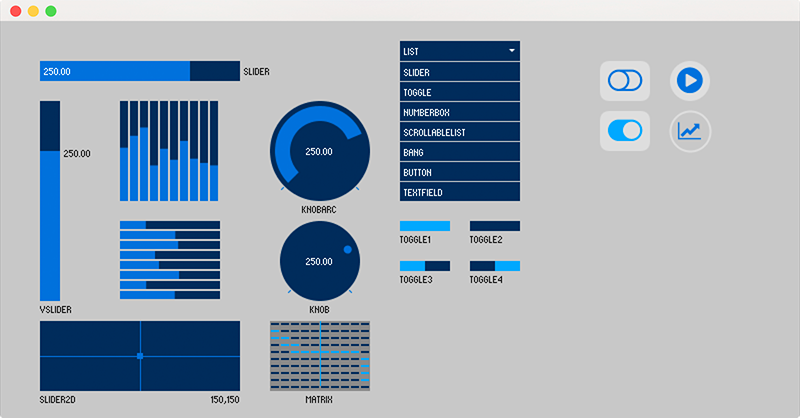
\includegraphics[width=1\textwidth]{imagenes/cp5_examples.png}
    \caption{Imagen con diferentes funcionalidades de ControlP5. Extraído de: \cite{cp5_image}}
\end{figure}

\subsection{Desarrollo de funciones secuenciales sin FREERTOS }

Una vez aprendidos los fundamentos de las herramientas a utilizar, y antes de implementarlas, se debe tener una idea general de las diferentes funciones a incluir en el sistema. Para comenzar con la programación, primero se realizarán de forma secuencial, sin utilizar FreeRTOS, y sin utilizar la comunicación serial. Se comprobará que el funcionamiento sea correcto antes de avanzar a la siguiente etapa. 

\subsection{Desarrollo de funciones concurrentes con FREERTOS}

En esta etapa se adaptarán las funciones desarrolladas anteriormente a FreeRTOS, y se incluirán las medidas pertinentes para asegurar que dichas funciones puedan trabajar de manera concurrente. Se comenzará a trabajar con el puerto serie para mostrar los valores de los sensores, pero sin representarlos de manera gráfica. Se comprobarán los tiempos de respuesta para asegurar que cumple las restricciones de tiempo real. 

\subsection{Desarrollo de interfaz de usuario base sin comunicaciones serie}

Se comenzará a crear la interfaz con Processing, de manera esquemática y sin comunicaciones con Arduino. Se comprobará que todos los módulos responden a los \textit{inputs} del usuario, así como la estructura de dichos módulos divididos en secciones para una mayor comodidad y comprensión.

\subsection{Desarrollo interfaz de usuario con comunicaciones serie}

Utilizando la interfaz base, se añadirá funcionalidad a todos los módulos y comunicación mediante puerto serie con Arduino. También se perfeccionará la interfaz en el aspecto visual. 

\subsection{Depuración, limpieza y documentación del código fuente}

Una vez desarrollada la interfaz de usuario y la programación del sistema, se depurará el código para solucionar los posibles errores que se hayan pasado por alto durante el desarrollo. También se reorganizará y optimizará el código para buscar una mayor eficiencia. 

Tras estos pasos, se realizará una documentación de cada una de las funciones del ámbito de Arduino y se añadirá el archivo de cabeceras. 

\subsection{Montaje en maqueta } 

Como última tarea, y si la temporización real lo permite, se implementará este sistema en una maqueta de un vehículo, que mostrará todas las funciones desarrolladas de una manera más realista en comparación al montaje en \textit{breadboard} que se ha realizado hasta el momento. 

\section{Temporización}


En esta temporización se consideran laborables los días de lunes a sábado, ambos incluidos. Se supone una media de trabajo de tres horas y media al día, sumando un total de veintiún horas a la semana. 

\begin{table}[H]
    \resizebox{\textwidth}{!}{%
    \begin{tabular}{|l|c|c|c|}
    \hline
    \rowcolor[HTML]{DAE8FC} 
    \multicolumn{1}{|c|}{\cellcolor[HTML]{DAE8FC}{\color[HTML]{000000} Tarea}} & {\color[HTML]{000000} \begin{tabular}[c]{@{}c@{}}Tiempo \\ estimado\end{tabular}} & Fecha de inicio & Fecha de finalización \\ \hline
    \textbf{Aprendizaje FreeRTOS} & 1/2 semana & 19/06/2023 & 21/06/2023 \\ \hline
    \textbf{Aprendizaje Processing} & 1/2 semana & 22/06/2023 & 24/06/2023 \\ \hline
    \textbf{Montaje de prototipo} & 3/2 semana & 26/06/2023 & 12/07/2023 \\ \hline
    \textbf{Funciones secuenciales} & 1/2 semana & 26/06/2023 & 28/06/2023 \\ \hline
    \textbf{Funciones concurrentes} & 2 semanas & 29/06/2023 & 12/07/2023 \\ \hline
    \textbf{Interfaz base} & 1 semana & 13/07/2023 & 15/07/2023 \\ \hline
    \textbf{Interfaz con serial} & 1 semana & 17/07/2023 & 23/07/2023 \\ \hline
    \textbf{\begin{tabular}[c]{@{}l@{}}Depuración, limpieza\\ y documentación\end{tabular}} & 1/2 semana & 24/07/2023 & 26/07/2023 \\ \hline
    \textbf{Montaje en maqueta} & 2 semanas & 27/07/2023 & 08/08/2023 \\ \hline
    \end{tabular}%
    }
    \caption[Temporización inicial]{Temporización estimada del proyecto. Elaboración propia}

    \end{table}

    \begin{figure}[h]
        \centering
        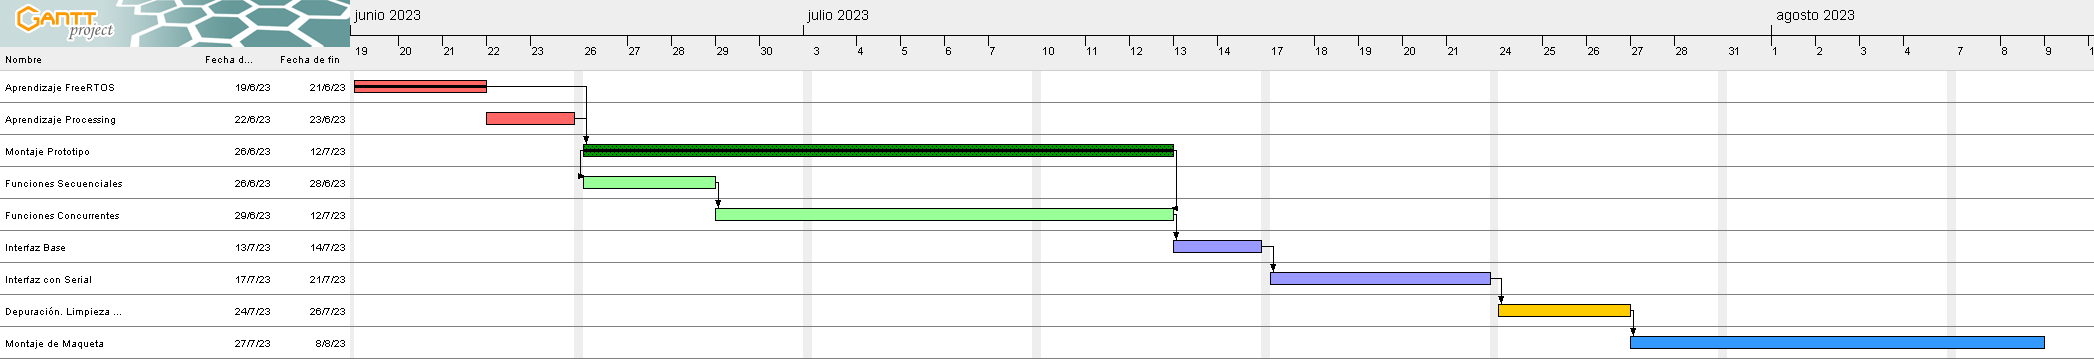
\includegraphics[width=1\textwidth]{imagenes/gantt_base.png}
        \caption{Diagrama de Gantt con las tareas temporizadas. Elaboración propia en GanttProject}
    \end{figure}
    

\section{Presupuesto}

A la hora de calcular el presupuesto necesario para el proyecto, debemos tener en cuenta tres factores principales: \textbf{coste del hardware}, \textbf{coste del software}, y el \textbf{coste de salarios} de los individuos implicados en el proyecto. Ninguno de estos es descartable ni se puede obviar, por lo que esta sección se desglosará en esas tres partes.
\subsection{Coste del hardware}

Al calcular el coste de los componentes que conforman el proyecto se han escogido los precios que se van a pagar en el momento de la planificación, los cuales pueden variar respecto al tiempo en el que se publique este trabajo. 


\begin{table}[H]
    \resizebox{\textwidth}{!}{%
    \begin{tabular}{|l|c|c|c|}
    \hline
    \rowcolor[HTML]{DAE8FC} 
    \multicolumn{1}{|c|}{\cellcolor[HTML]{DAE8FC}{\color[HTML]{000000} \textbf{Componente}}} & \textbf{Unidades} & \textbf{Precio sin I.V.A} & \textbf{Precio con I.V.A} \\ \hline
    \textbf{Placa Arduino Mega 2560 R3 (clon)} & 1 ud & 20,90€ & 26,45€ \\ \hline
    \textbf{LEDs variadas (25 uds)} & 25 uds & 1,98€ & 2,50€ \\ \hline
    \textbf{Resistencias variadas (50 uds)} & 50 uds & 1,98€ & 2,50€ \\ \hline
    \textbf{Batería 9V 650mAh Li-ion} & 2 uds & 21,32€ & 26,99€ \\ \hline
    \textbf{Motor DC} & 2 uds & 7,82€ & 9,90€ \\ \hline
    \textbf{Módulo L298N} & 1 ud & 3,94€ & 4,99€ \\ \hline
    \textbf{Termistor 10k} & 2 uds & 3,15€ & 3,99€ \\ \hline
    \textbf{Cables M-M, M-F, F-F} & 100 uds & 1,98€ & 2,50€ \\ \hline
    \textbf{Maqueta coche Mustang Shelby} & 1 ud & 28,43€ & 35,99€ \\ \hline
    \textbf{Cable USB-A a USB-B de 2 metros} & 1 ud & 7,81€ & 9,99€ \\ \hline
    \multicolumn{2}{|l|}{\textbf{Total}} & 99,31€ & 125,8€ \\ \hline
    \end{tabular}%
    }
    \caption[Presupuesto de componentes]{Lista de componentes con coste. Elaboración propia}

    \end{table}


\subsection{Coste del software}

En esta sección se describirán los costes de los programas utilizados, aunque al darse prioridad al software libre y gratuito, el coste de estas herramientas siempre será cero, exceptuando Windows por la necesidad de este sistema operativo en el ordenador que se está utilizando para otras funciones.

\begin{table}[H]
    \resizebox{\textwidth}{!}{%
    \begin{tabular}{|l|c|l|l|c|}
    \cline{1-2} \cline{4-5}
    \multicolumn{1}{|c|}{\cellcolor[HTML]{DAE8FC}{\color[HTML]{000000} \textbf{Programa / Recurso}}} & \cellcolor[HTML]{DAE8FC}\textbf{Precio licencia} &  & \cellcolor[HTML]{DAE8FC}{\color[HTML]{000000} \textbf{Programa / Recurso}} & \multicolumn{1}{l|}{\cellcolor[HTML]{DAE8FC}{\color[HTML]{000000} \textbf{Precio licencia}}} \\ \cline{1-2} \cline{4-5} 
    \textbf{Arduino IDE} & 0€ &  & \textbf{TexLive} & 0€ \\ \cline{1-2} \cline{4-5} 
    \textbf{FreeRTOS} & 0€ &  & \textbf{GIMP} & 0€ \\ \cline{1-2} \cline{4-5} 
    \textbf{Processing} & 0€ &  & \textbf{GitHub} & 0€ \\ \cline{1-2} \cline{4-5} 
    \textbf{Visual Studio Code} & 0€ &  & \textbf{Mozilla Firefox} & 0€ \\ \cline{1-2} \cline{4-5} 
    \textbf{Atom} & 0€ &  & \textbf{Licencia Windows} & 18€ \\ \cline{1-2} \cline{4-5} 
    \textbf{Tinkercad} & 0€ & & &  \\ \cline{1-2} \cline{4-5}
    \end{tabular}%
    }
    \caption[Presupuesto de software]{Lista de software utilizado con coste. Elaboración propia}
    \end{table}


\subsection{Coste de salarios}

Una vez hallados los costes de software y hardware, se debe estimar el coste dedicado a remunerar los servicios de los diferentes integrantes humanos del proyecto. 

Los salarios medios se han extraído de la plataforma GlassDoor, con lo que se ha calculado el salario por hora de los puestos, asumiendo que dichos puestos estuvieran activos un total de cuarenta horas a la semana, cuatro semanas por mes, durante doce meses. 

\begin{table}[H]
    \resizebox{\textwidth}{!}{%
    \begin{tabular}{|l|l|l|l|l|l|}
    \hline
    \rowcolor[HTML]{DAE8FC} 
    \multicolumn{1}{|c|}{\cellcolor[HTML]{DAE8FC}{\color[HTML]{000000} \textbf{Puesto de trabajo}}} & \multicolumn{1}{c|}{\cellcolor[HTML]{DAE8FC}\textbf{\begin{tabular}[c]{@{}c@{}}Salario\\  por hora\end{tabular}}} & \multicolumn{1}{c|}{\cellcolor[HTML]{DAE8FC}{\color[HTML]{000000} \textbf{\begin{tabular}[c]{@{}c@{}}Horas por\\ semana\end{tabular}}}} & \multicolumn{1}{c|}{\cellcolor[HTML]{DAE8FC}\textbf{\begin{tabular}[c]{@{}c@{}}Semanas\\  de Trabajo\end{tabular}}} & \multicolumn{1}{c|}{\cellcolor[HTML]{DAE8FC}\textbf{\begin{tabular}[c]{@{}c@{}}Total\\ de horas\end{tabular}}} & \multicolumn{1}{c|}{\cellcolor[HTML]{DAE8FC}\textbf{\begin{tabular}[c]{@{}c@{}}Salario\\ Total\end{tabular}}} \\ \hline
    \textbf{\begin{tabular}[c]{@{}l@{}}Ingeniero de\\ Sistemas Empotrados\end{tabular}} & 17,19€/h & 21 horas & 7,5 sem & 157,5 horas & 2707,42€ \\ \hline
    \textbf{\begin{tabular}[c]{@{}l@{}}Desarrollador de \\ interfaces de usuario\end{tabular}} & 14,73€/h & 21 horas & 2 sem & 42 horas & 618,66€ \\ \hline
    \end{tabular}%
    }

    \caption[Presupuesto de salarios]{Lista de salarios requeridos para el proyecto. Elaboración propia}

    \end{table}


	% Desarrollo bajo sprints: 
	% 	1. Permitir registros y login de usuarios
	% 	2. Desarrollo del sistema de incidencias
	% 	3. Desarrollo del sistema de denuncias administrativas y accidentes
	% 	4. Desarrollo del sistema de croquis
	%   5. Instalación de la aplicación de manera automática
	\chapter{Análisis del problema}

\fancyhead[R]{6. Análisis del problema}

\noindent\fbox{
	\parbox{\textwidth}{
    En este capítulo se realizará un análisis algo más exhaustivo de la toma de diversas decisiones que afectarán al desarrollo del trabajo, véase los componentes, el sistema operativo de tiempo real, y demás componentes que conforman el proyecto y desarrollo. 
	}
}

\section{Elección de un sistema operativo}

\subsection{¿SO de propósito general o sistema operativo de tiempo real?}

El principal rol del sistema operativo es controlar los recursos del sistema para suplir las demandas de las aplicaciones que trabajan sobre él. Todos los SOs, independientemente de si son de propósito general o de tiempo real, tienen elementos esenciales tales como la planificación de procesos, control de memoria, relojes, entrada/salida, etcétera. 

Si bien comparten dichos elementos esenciales, los RTOS están diseñados con la filosofía de que sus tiempos de espera, procesamiento y respuesta son más importantes que su rendimiento promedio. Los RTOS se utilizan en los casos en los procesos deban estar planificados en el tiempo, garantizando que se cumplan los requerimientos temporales para dichos procesos. 

En el caso de este proyecto, se necesita que el SO a escoger tenga baja latencia, que pueda asegurar que las tareas que lo requieran terminarán en el tiempo determinado, así como permitir que las tareas críticas y no críticas coexistan en el sistema. También es muy importante que dicho SO tenga un sistema de asignación de prioridades que permita al programador establecer cuáles son las tareas y procesos más importantes para su proyecto y darles esa importancia en la ejecución.

\subsection{¿RTOS comercial o de código abierto?}

Si bien los RTOS comerciales ofrecen una mayor variedad de funciones para el programador, sus precios suelen ser demasiado elevados para poder escogerlos en un proyecto como este. Por ejemplo, en el caso de VxWorks, el RTOS propietario líder en el sector, de la empresa Wind River, el precio del SO comienza en los 18500\$ per seat (por usuario que trabaja con el sistema). Obviamente esto es algo prohibitivo para nuestro presupuesto, pero en el caso de una ECU que se implemente en vehículos sería la mejor opción.\newline

Pero no todos los RTOS son comerciales, sino que existen multitud de ellos que son de código abierto. A continuación se expone una tabla con las principales características de algunos de los RTOS \textit{open source} más importantes:

\begin{table}[H]
    \resizebox{\columnwidth}{!}{%
    \begin{tabular}{|l|l|l|l|}
    \hline
    \rowcolor[HTML]{CBCEFB} 
    \textbf{Nombre} &
      \textbf{Aplicación principal} &
      \textbf{\begin{tabular}[c]{@{}l@{}}Facilidad de \\ programación\end{tabular}} &
      \textbf{\begin{tabular}[c]{@{}l@{}}Eficiencia en \\ ECU\end{tabular}} \\ \hline
    \textbf{RIOT}        & \begin{tabular}[c]{@{}l@{}}Orientado a dispositivos de\\  Internet de las Cosas (IoT)\end{tabular} & Media   & Media \\ \hline
    \textbf{Nano-RK}     & \begin{tabular}[c]{@{}l@{}}Sistemas embebidos en\\ tiempo real\end{tabular}                        & Difícil & Alta  \\ \hline
    \textbf{FreeRTOS}    & \begin{tabular}[c]{@{}l@{}}Sistema operativo de tiempo\\  real de código abierto\end{tabular}      & Media   & Media \\ \hline
    \textbf{ARM mbed OS} & Plataforma de desarrollo para IoT                                                                  & Fácil   & Alta  \\ \hline
    \textbf{Raspbian}    & \begin{tabular}[c]{@{}l@{}}Sistema operativo general\\  para Raspberry Pi\end{tabular}             & Fácil   & Baja  \\ \hline
    \textbf{DuinOS}      & \begin{tabular}[c]{@{}l@{}}RTOS diseñado específicamente\\  para Arduino\end{tabular}              & Fácil   & Baja  \\ \hline
    \textbf{mipOS}       & \begin{tabular}[c]{@{}l@{}}RTOS de código abierto para\\  sistemas embebidos\end{tabular}          & Media   & Baja  \\ \hline
    \end{tabular}%
    }
    \caption[Selección de RTOS]{Lista de sistemas de tiempo real y sus características. Elaboración propia}

    \end{table}

Para escoger, comenzamos por descartar todos aquellos sistemas operativos que se utilicen para IoT, pues normalmente las restricciones de tiempo en esos sistemas son mucho más suaves. Si hacemos un balance entre la facilidad de programación y la eficiencia, pues el tiempo de desarrollo es bastante limitado y diseñar un programa en los sistemas más difíciles puede requerir demasiado tiempo, encontramos que la mejor alternativa es FreeRTOS. 

\subsubsection{FreeRTOS}

FreeRTOS es uno de los RTOS más utilizados para microcontroladores y pequeños microprocesadores, con soporte para una gran variedad de placas\cite{freertos}. Tiene una proyección \textbf{LTS} (\textit{Long Term Support}), lo que garantiza que el proyecto podrá seguir teniendo soporte a largo plazo. Una de sus grandes ventajas es la gran cantidad de librerías modulares, así como también el enfoque del kernel para ahorrar energía y no ser demasiado pesado. 

Por todas estas razones, FreeRTOS es la elección perfecta para un proyecto con estas características. 

\section{Elección de la placa}
\subsection{Requisitos}
A la hora de escoger la placa existen varios requisitos básicos debe cumplir, nombrados a continuación: 

\subsubsection{Soporte de FreeRTOS}

El primer requisito es que FreeRTOS soporte la placa que vayamos a escoger. Por suerte, este SO está ampliamente compatibilizado y existen multitud de placas disponibles\cite{freertos_comp}. Entre ellos están las placas de Altera, Infineon, Raspberry Pi, e incluso los usuarios han desarrollado FreeRTOS compatible con Arduino.

\subsubsection{Precio}

Si bien algunas de las placas anteriormente nombradas son objetivamente mejores, el presupuesto es limitado y requerimos de una placa que, como precio máximo, cueste 50\$. Con esto descartamos las placas de Altera e Infineon, así como una gran multitud de marcas que están orientadas a proyectos de ámbito profesional. 

\subsubsection{Rendimiento y frecuencia de reloj}

Al ser un proyecto con RTOS, se necesita que la placa tenga una frecuencia de reloj que permita realizar las funciones más importantes en un periodo corto, incluso en el peor caso. Para comenzar con la estimación, debemos destacar aquellas funciones del sistema que tengan el plazo más restrictivo. 

En el caso de la comprobación de la temperatura de batería y motor, debe de medirse dicha temperatura cada muy poco tiempo, asegurando así que el sistema no se esté sobrecalentando y pueda provocar un problema. 

Para realizar dichas mediciones, tendremos en cuenta dos funciones necesarias. 

\begin{enumerate}
    \item Inicio del sensor: Los sensores que se utilizan para medir temperaturas tienen un tiempo mínimo de 1s para conseguir la temperatura correcta, por lo que se iniciará y, un segundo después, se avisará a la segunda función.
    \item Comprobación de la temperatura: La ECU leerá los valores que le ha mandado el sensor en el último segundo y, mediante una ecuación, hallará el valor en grados celsius correspondiente. Tras hacer esto, comparará el valor con el límite superior que definen el intervalo de temperaturas correctas y, si no está dentro de dichos valores, enviará una señal a otra función que mostrará el aviso de temperatura por pantalla. 
\end{enumerate}

La segunda función es la que nos marcará el mínimo valor necesario de frecuencia de reloj para que el sistema pueda funcionar correctamente, realizando mediciones cada 100 ms. Para poder hallar entonces cuál es ese valor, programamos con pseudocódigo de manera básica una función que realice el proceso:


Se ha tomado como referencia un sensor LM35 cuya ecuación para hallar la temperatura es la siguiente: 

\begin{verbatim}
    Temperatura = Valor * 5 * 100 /1024
\end{verbatim}


\begin{verbatim}
    subproceso funcion temperatura_bateria
        tempB <- leer(sensor)
        temB <- (tempB * 5 * 100) / 1024
        si tempB > 45
            entonces temp_error = 1
        fin si
    fin funcion
\end{verbatim}

Teniendo ya este pseudocódigo, podemos estimar de manera aproximada la cantidad de ciclos y las instrucciones necesarias para llevar a cabo esta función, por lo que necesitamos convertir este código a ensamblador: 

\begin{verbatim}
    LDR rdi, #SENSOR 
    MUL $0.48828125, rdi
    CMP rdi, $45
    JA .L1
    MOV $1, rsi

    .L1
\end{verbatim}

Por motivos de eficiencia se ha reducido la operación de la fórmula al mínimo posible. 

Teniendo en cuenta que la operación que mayor número de cicos necesita, que es LOAD, con cinco ciclos, vamos a aproximar el número de ciclos del resto de instrucciones a 5 para poseer mayor margen en el cálculo a la hora de escoger la frecuencia de reloj necesaria.

Por tanto, nuestro programa tardará como mínimo 5 * 5 = 25 ciclos de reloj.

Ahora, teniendo en cuenta lo aprendido en la asignatura de Arquitectura de Computadores, vamos a hallar la frecuencia de reloj mínima para que el sistema pueda realizar este proceso en el tiempo determinado de 10ms. Utilizaremos la siguiente fórmula: 

\begin{align*}
    T_{CPU} = NI * CPI * T_{CICLO}
\end{align*}

Añadiendo los datos que conocemos, resolvemos la ecuación:

\begin{align*}
    100ms = 5 * 5 * T_{CICLO} 
\end{align*}

\begin{align*}
    \frac{100}{25} = T_{CICLO}
\end{align*}


\begin{align*}
    T_{CICLO} = 4ms
\end{align*}

Si calculamos la inversa del tiempo de ciclo, obtenemos la frecuencia mínima a la que debe operar nuestra placa para poder cumplir con los requerimientos:\newline
\begin{align*}
    Frecuencia > \frac{1}{0.04s}
\end{align*}

\begin{align*}
    Frecuencia > 2.5kHz
\end{align*}

\subsubsection{Periféricos}

Por último, se valorará que la placa tenga los siguientes parámetros:

\begin{itemize}
    \item Número de entradas/salidas digitales
    \item Salidas analógicas con \textbf{PWM} (pulse width modulation)
    \item Comunicación \textbf{I2C}(Inter-Integrated Circuit)
    \item Puertos serie
\end{itemize}



\subsubsection{Conclusiones}

Una vez analizados los puntos más importantes, se ha seleccionado una variedad de placas que cumplen uno o varios requisitos nombrados. 

\begin{table}[H]
    \resizebox{\columnwidth}{!}{%
    \begin{tabular}{|l|l|l|l|l|l|l|l|}
    \hline
    \rowcolor[HTML]{ECF4FF} 
    \textbf{Nombre} &
      \textbf{Empresa} &
      \textbf{\begin{tabular}[c]{@{}l@{}}Frecuencia \\ Reloj\end{tabular}} &
      \textbf{RAM} &
      \textbf{\begin{tabular}[c]{@{}l@{}}Utilidades \\ Incluidas\end{tabular}} &
      \textbf{\begin{tabular}[c]{@{}l@{}}Soporta \\ FreeRTOS\end{tabular}} &
      \textbf{\begin{tabular}[c]{@{}l@{}}Temperatura \\ de Operación\end{tabular}} &
      \textbf{PVP} \\ \hline
    \textbf{Arduino Mega 2560} &
      Arduino &
      16 MHz &
      8 KB &
      \begin{tabular}[c]{@{}l@{}}UART, SPI, I2C, \\ PWM, ADC\end{tabular} &
      Sí* &
      -40°C a 85°C &
      40\$ \\ \hline
    \textbf{Raspberry Pi 4} &
      \begin{tabular}[c]{@{}l@{}}Raspberry Pi\\  Foundation\end{tabular} &
      1.5 GHz &
      4 GB &
      \begin{tabular}[c]{@{}l@{}}GPIO, UART, \\ SPI, I2C, PWM, \\ ADC\end{tabular} &
      Sí &
      0°C a 50°C &
      45\$ \\ \hline
    \textbf{\begin{tabular}[c]{@{}l@{}}BeagleBone \\ Black\end{tabular}} &
      BeagleBoard.org &
      1 GHz &
      512 MB &
      \begin{tabular}[c]{@{}l@{}}GPIO, UART, \\ SPI, I2C, ADC\end{tabular} &
      Sí &
      -20°C a 85°C &
      55\$ \\ \hline
    \textbf{Teensy 4.1} &
      PJRC &
      600 MHz &
      1024 KB &
      \begin{tabular}[c]{@{}l@{}}UART, SPI, I2C, \\ PWM, ADC\end{tabular} &
      Sí &
      -40°C a 85°C &
      32\$ \\ \hline
    \textbf{\begin{tabular}[c]{@{}l@{}}STM32 \\ Nucleo-F767ZI\end{tabular}} &
      STMicroelectronics &
      216 MHz &
      512 KB &
      \begin{tabular}[c]{@{}l@{}}UART, SPI, I2C, \\ PWM, ADC\end{tabular} &
      Sí &
      -40°C a 85°C &
      52\$ \\ \hline
    \textbf{\begin{tabular}[c]{@{}l@{}}NVIDIA \\ Jetson Nano\end{tabular}} &
      NVIDIA &
      1.43 GHz &
      4 GB &
      \begin{tabular}[c]{@{}l@{}}GPIO, UART, \\ SPI, I2C, USB, \\ Ethernet, HDMI\end{tabular} &
      Sí &
      0°C a 50°C &
      99\$ \\ \hline
    \textbf{\begin{tabular}[c]{@{}l@{}}PSoC 6 \\ BLE Pioneer Kit\end{tabular}} &
      \begin{tabular}[c]{@{}l@{}}Cypress \\ Semiconductor\end{tabular} &
      150 MHz &
      1 MB &
      \begin{tabular}[c]{@{}l@{}}UART, SPI, I2C, \\ PWM, ADC\end{tabular} &
      No &
      -40°C a 85°C &
      49\$ \\ \hline
    \end{tabular}%
    }
    \caption[Selección de placa]{Lista de placas seleccionadas y sus características. Elaboración propia}

    \end{table}

    Teniendo en cuenta esta tabla, comenzamos a descartar aquellos que superen el presupuesto inicial de 50\$. Después, aquellas que no tengan soporte para FreeRTOS. La elección final, entre la placa Teensy y la arduino mega, es mayormente por la documentación y el soporte que tengan las placas. Se ha escogido la \textbf{Arduino Mega 2560} porque, además de dicha documentación, facilita el montaje del prototipo gracias a sus pines, evitando así la necesidad de soldar ni de una protoboard.


    \begin{figure}[H]
        \centering
        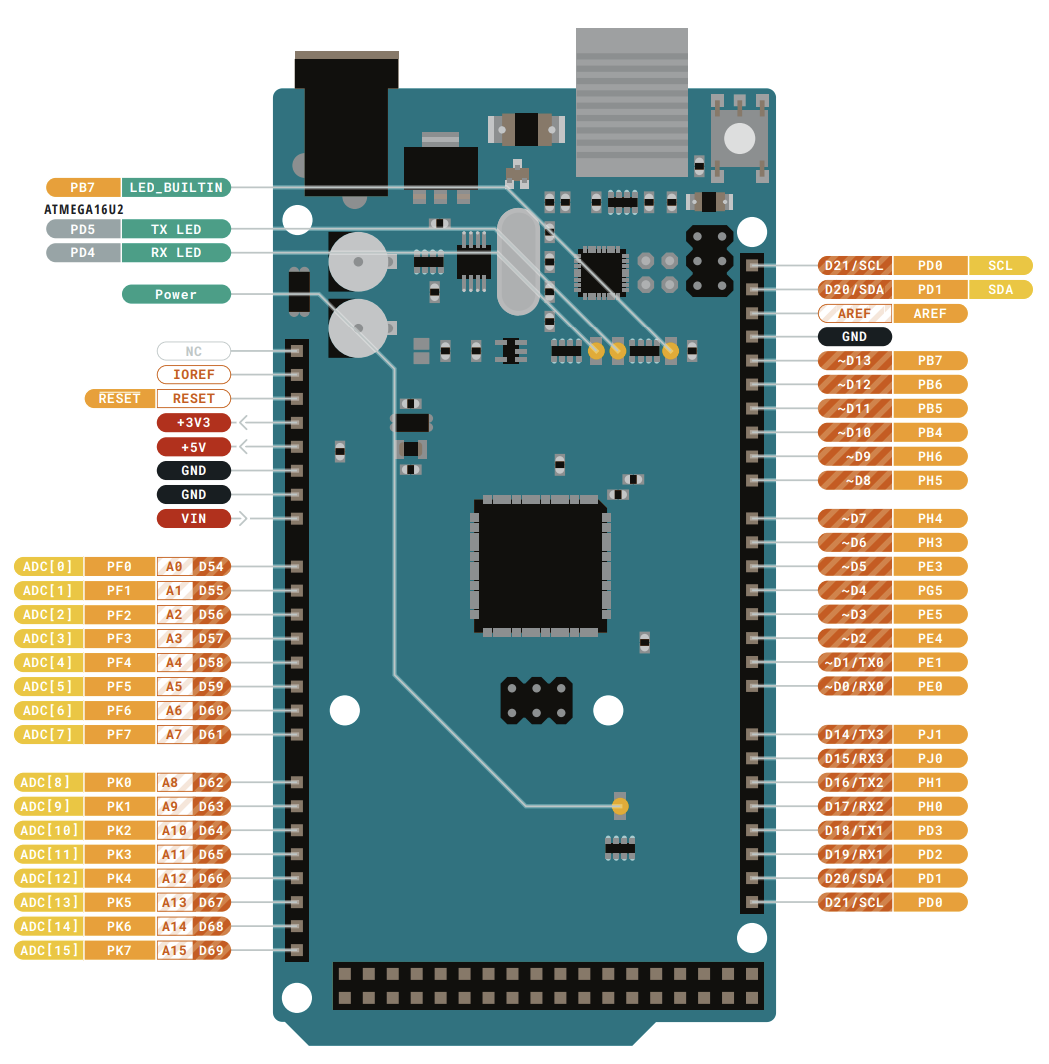
\includegraphics[width=1\textwidth]{imagenes/pinout_amega2560.png}
        \caption{Esquema de pines de la Arduino Mega 2560. Extraído de: \cite{arduino_mega}}
    \end{figure}
 

\section{Elección de periféricos}
 
Si bien no es una parte tan importante de la selección de componentes, escoger un buen periférico puede facilitar las labores de montaje y programación. No todos los periféricos pueden ser válidos en este proyecto, pues existen restricciones de precio y tamaño, por lo que se tiene que tener en cuenta estos parámetros a la hora de escoger. 



 \subsection{Motor}

 En el caso de los motores, existen tres tipos principales: 

 \begin{enumerate}
  \item Motores DC: Son los más utilizados, aunque pueden requerir de un módulo de control o un puerto PWM para poder ser manejados con eficiencia.
  \item Motores paso a paso: Giran mediante pasos, siendo 1.8º y 3.75º las medidas más usuales. Requieren de un módulo para controlar su manejo.
  \item Servomotores: Son motores que únicamente pueden dar un giro de 180º, pero proporcionan un control total del giro.
 \end{enumerate}

 En este caso, la elección ha sido clara, los motores DC cumplen con todo lo necesario y además existen multitud de modelos. 
 Se ha escogido un motor básico, con eje para conectarse a la rueda, y se comprarán dos unidades para las dos ruedas delanteras del vehículo. 

 \subsubsection{Placa de control de motor}

 Entre las dos alternativas más utilizadas, el driver L298H, con una capacidad para dos motores DC, y el escudo L293D, de la empresa MH Electronics, se ha escogido el primero debido a haber trabajado con el anteriormente y conocer su funcionamiento, además de ser apto para los dos motores DC necesarios. 

 \begin{figure}[H]
  \centering
  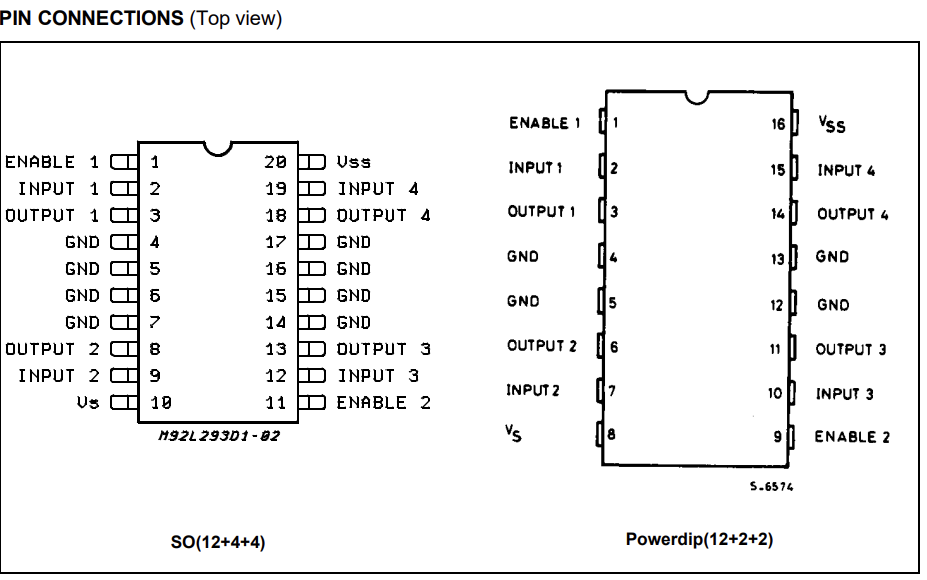
\includegraphics[width=1\textwidth]{imagenes/pinout_L293D.png}
  \caption{Esquema de pines del Shield L293D. Extraído de: [27]}
\end{figure}

 \subsection{Sensores de temperatura}

 Respecto a los sensores de temperatura, se ha escogido el termistor MF52 de 10K Ohm, debido a su bajo coste y su buena precisión.
 Se comprarán dos, uno para la temperatura del motor y otro para la batería.

 \subsection{Batería}

 Como elección de las baterías, se ha escogido un pack de dos baterías recargables ENEGON, de 9 voltios y 650 miliamperios/hora, suficiente para suministrar energía a los motores. Además, es recargable por usb para una mayor utilidad.
 
\section{Componentes en situaciones reales}

Si bien estos componentes cumplen las necesidades del proyecto, nunca serían útiles en un entorno real. Esta ECU es una abstracción de una ECU real, en la que tendríamos que tener en cuenta muchos más factores tales como la temperatura, mayor fiabilidad en los sistemas, así como el resto de requerimientos que tendría un vehículo real, incluyendo un motor de gasolina que complicaría el sistema y conlleva multitud de riesgos. Además, los componentes que se utilizarían en un entorno real rondan los miles de euros, por lo que no es posible realizar un proyecto realista. 
	% Análisis del problema
	% 1. Análisis de requisitos
	% 2. Análisis de las soluciones
	% 3. Solucion propuesta
	% 4. Análisis de seguridad

	\chapter{Implementación}

La implementación del software se ha dividido en hitos. Estos, han sido definidos en Github
y cada uno de ellos contiene un grupo de \textit{issues} que se corresponden con las distintas
mejoras que se han ido incorporando al software a lo largo de su desarrollo.\\



	% Trabajos futuros

	\chapter{Conclusiones y trabajos futuros}




	
	\newpage
	\bibliography{bibliografia}
	\bibliographystyle{plain}
	
\end{document}

